\documentclass[11pt]{report}
% Load packages
\usepackage[a4paper,width=150mm,top=25mm,bottom=25mm]{geometry} %todo: Get correct margin
\usepackage[english]{babel}
\usepackage[dvipsnames]{xcolor}     % More colors
\usepackage[backref=page]{hyperref} % Clickable links in PDF (must be loaded before cleveref and glossaries)
\usepackage{amsmath}			    % Math
\usepackage{amssymb}			    % More math
\usepackage{booktabs}			    % Neat tables
\usepackage{fancyhdr}			    % Customize header and footers
\usepackage{float}				    % Floating figures / tables
\usepackage[symbols,acronyms,
    abbreviations,automake]
    {glossaries-extra}              % Allows for definition of acronyms, symbols and stuff
\usepackage{graphicx}			    % Pictures / Graphics
\usepackage{cleveref}               % Automatically add prefix to reference (e.g. fig. if figure)
\usepackage{listings}			    % Typeset programming languages
\usepackage{microtype}              % Overall improvement of formatting
\usepackage{multirow}               % Table entries over multiple columns
\usepackage{pdfpages}			    % Allows for inclusion of pdf files
\usepackage{physics}			    % Vector stuff
\usepackage{siunitx}			    % SI Units
\usepackage{subcaption}             % Subfigure captions
\usepackage{standalone}			    % Used for TikZ code outsourcing
\usepackage{tikz}				    % Powerful drawing tool for latex
\usepackage{tikz-3dplot}            % TikZ 3D
\usepackage{tikz-dimline}		    % Dimension (measure) lines for TikZ
\usepackage{titlesec}               % Allows for different title styles, but also allows for full gls every chapter
\usepackage[nottoc]{tocbibind}      % nottoc means do not show toc in toc
\usepackage{todonotes}			    % Todo commands

% Load tikz libraries, styles and commands
% Load additional tikz libraries
\usetikzlibrary{angles, arrows, calc, decorations.pathmorphing, quotes, shapes.geometric, snakes, spy}

%% Define tikz shapes and styles
% Flow chart
\tikzstyle{startstop} = [rectangle, rounded corners, minimum width=3cm, minimum height=1cm,text centered, draw=black, fill=red!30]
\tikzstyle{io} = [trapezium, trapezium left angle=70, trapezium right angle=110, minimum width=3cm, minimum height=1cm, text centered, draw=black, fill=blue!30]
\tikzstyle{process} = [rectangle, minimum width=3cm, minimum height=1cm, text centered, text width=3.5cm, draw=black, fill=orange!30]
\tikzstyle{decision} = [diamond, aspect=3, minimum width=3cm, minimum height=1cm, text centered, draw=black, fill=green!30]
\tikzstyle{arrow} = [thick,->,>=stealth]

% 3D coordinate system rotation
\newcommand{\rotateRPY}[3]% roll, pitch, yaw
{   \pgfmathsetmacro{\rollangle}{#1}
    \pgfmathsetmacro{\pitchangle}{#2}
    \pgfmathsetmacro{\yawangle}{#3}
    
    % to what vector is the x unit vector transformed, and which 2D vector is this?
    \pgfmathsetmacro{\newxx}{cos(\yawangle)*cos(\pitchangle)}
    \pgfmathsetmacro{\newxy}{sin(\yawangle)*cos(\pitchangle)}
    \pgfmathsetmacro{\newxz}{-sin(\pitchangle)}
    \path (\newxx,\newxy,\newxz);
    \pgfgetlastxy{\nxx}{\nxy};
    
    % to what vector is the y unit vector transformed, and which 2D vector is this?
    \pgfmathsetmacro{\newyx}{cos(\yawangle)*sin(\pitchangle)*sin(\rollangle)-sin(\yawangle)*cos(\rollangle)}
    \pgfmathsetmacro{\newyy}{sin(\yawangle)*sin(\pitchangle)*sin(\rollangle)+ cos(\yawangle)*cos(\rollangle)}
    \pgfmathsetmacro{\newyz}{cos(\pitchangle)*sin(\rollangle)}
    \path (\newyx,\newyy,\newyz);
    \pgfgetlastxy{\nyx}{\nyy};
    
    % to what vector is the z unit vector transformed, and which 2D vector is this?
    \pgfmathsetmacro{\newzx}{cos(\yawangle)*sin(\pitchangle)*cos(\rollangle)+ sin(\yawangle)*sin(\rollangle)}
    \pgfmathsetmacro{\newzy}{sin(\yawangle)*sin(\pitchangle)*cos(\rollangle)-cos(\yawangle)*sin(\rollangle)}
    \pgfmathsetmacro{\newzz}{cos(\pitchangle)*cos(\rollangle)}
    \path (\newzx,\newzy,\newzz);
    \pgfgetlastxy{\nzx}{\nzy};
}
\tikzset{RPY/.style={x={(\nxx,\nxy)},y={(\nyx,\nyy)},z={(\nzx,\nzy)}}}
% Graphic paths
\graphicspath{{Graphics/}
            {Graphics/ExperimentalSetup/}
            {Graphics/Methods/}
            {Graphics/Background/}
            {Graphics/Results/}
            {Graphics/TikZ}}

% Formatting settings
\pagestyle{fancy}				% Activate fancy style
\setlength{\headheight}{15pt}	% To prevent warning
\setlength\parindent{0pt}		% No indentation when starting new paragraph
\setcounter{secnumdepth}{4}     % Level to which (sub)sections are numbered
\setcounter{tocdepth}{3}        % Level to which (sub)sections are displayed in toc
% \fancyhead[<position specifiers>]{<text>} and same for fancyfoot
% pos specifier: left (L), right (R), centre (C), odd (O), even (E) pages
% e.g. [RO, LE] means right on odd pages and left on even pages
% text specifier: pageNum (\thepage), chapter (\thechapter)

% Customize package settings
\pgfplotsset{compat=1.15}		% Use old version to prevent warning
\pdfminorversion=7				% PDF version 1.7
% Write full acronym again for every new chapter
\titleformat{\chapter}[display]
    {\normalfont\huge\bfseries}
    {\chaptertitlename\ \thechapter}
    {20pt}{\Huge}[\glsresetall]
% SI Units
% \sisetup{range-phrase=--}		% - instead of to, e.g. "1-7 nm" instead of "1 to 7 nm "
% \sisetup{range-units=single}	% Only one unit after second value (and none after first)
\sisetup{per-mode=fraction}
\renewcommand{\arraystretch}{1.2} % Increase space between rows in tables
\renewcommand*{\backref}[1]{}
\renewcommand*{\backrefalt}[4]{{\footnotesize [%
    \ifcase #1 Not cited.%
	\or Cited on page~#2%
	\else Cited on pages #2%
	\fi%
]}}
\renewcommand*{\glstextformat}[1]{\textcolor{black}{#1}}
% Change hyperlink colors
\definecolor{winered}{rgb}{0,0,128}
\hypersetup{
  colorlinks   = true, %Colours links instead of ugly boxes
  urlcolor     = blue, %Colour for external hyperlinks
  linkcolor    = RoyalPurple, %Colour of internal links
  citecolor   = OliveGreen %Colour of citations
}

% My own commands
\newcommand{\subInd}[1]{_\mathrm{#1}}
% Note todo in an own line
\newcommand{\itodo}[1]{\todo[inline]{#1}}
% Note improvement
\newcommand{\iimprov}[1]{\todo[inline, color=yellow!40]{#1}}
% Note questions
\newcommand{\iquest}[1]{\todo[inline, color=green!40]{#1}}
% Note suggestions
\newcommand{\isug}[1]{\todo[inline, color=blue!40]{#1}}
% Note todo in an own line but itemize possible
\newcommand{\todoin}[2][]{\todo[inline, caption={2do}, #1]{
		\begin{minipage}{\textwidth-4pt}#2\end{minipage}}}
\newcommand{\todoFig}[1]{\\\color{red}{\textbf{TODO: }}#1}
% Vector #1 in coordinate frame #2
\newcommand{\vincs}[2]{\ensuremath{{}_{\mathcal{\MakeUppercase{#2}}}\mathbf{{#1}}}}
% Quaternion to transform from cs #1 to cs #2
\newcommand{\qtf}[2]{\ensuremath{{}_{\mathcal{\MakeUppercase{#2}}}^{\mathcal{\MakeUppercase{#1}}}{\vb{q}}}}
% Rotation matrix to transform from cs #1 to cs #2
\newcommand{\mtf}[2]{\ensuremath{{}_{\mathcal{\MakeUppercase{#2}}}^{\mathcal{\MakeUppercase{#1}}}\mathbf{{M}}}}

% Start document and load all parts
\makeglossaries

% Acronyms
% First mention long, others short
\setabbreviationstyle[acronym]{long-short}
\newacronym{imu}{IMU}{Intertial Measurement Unit}
\newacronym{lidar}{LiDAR}{Light Detection And Ranging}
\newacronym{mems}{MEMS}{Microelectromechanical Systems}
\newacronym{ahrs}{AHRS}{Attitude Heading Reference System}
\newacronym{fov}{FOV}{Field Of View}
\newacronym{sonar}{SONAR}{Sound Navigation And Ranging}
\newacronym{radar}{RADAR}{Radio Detection And Ranging}
\newacronym{gps}{GPS}{Global Positioning System}
\newacronym{fir}{FIR}{Finite Impulse Response}
\newacronym{iir}{IIR}{Infinite Impulse Response}
\newacronym{ransac}{RANSAC}{Random Sample Consensus}
\newacronym{slam}{SLAM}{Simultaneous Localization and Mapping}
\newacronym{avp}{AVP}{Automated Valet Parking}
\newacronym{esp}{ESP}{Electronic Stabilzation Program}
\newacronym{abs}{ABS}{Anti-Lock Braking System}
\newacronym{ros}{ROS}{Robotic Operation System}
\newacronym{rmse}{RMSE}{Root-Mean-Square Error}
\newacronym{lpf}{LPF}{Low-Pass Filter}
\newacronym{hpf}{HPF}{High-Pass Filter}
\newacronym{tp}{TP}{True Positive}
\newacronym{fp}{FP}{False Positive}
\newacronym{kpi}{KPI}{Key Performance Indicator}
\newacronym{cnn}{CNN}{Convolutional Neural Network}
\newacronym{rcnn}{R-CNN}{Region Based Convolutional Neural Network}
\newacronym{roi}{ROI}{Region of interest}

% Symbols
\glsxtrnewsymbol[description={Vector}]{v}{$\vb{v}$}
\glsxtrnewsymbol[description={Unit vector}]{v_uv}{$\vu{v}$}
\glsxtrnewsymbol[description={Norm of vector}]{v_norm}{$\norm{v}$}
\glsxtrnewsymbol[description={Vector in coordinate frame $\mathcal{A}$}]{v2}{\vincs{v}{a}}
\glsxtrnewsymbol[description={Rotation matrix to transform from a to b}]{R}{\mtf{a}{b}}
\glsxtrnewsymbol[description={Quaternion to transform from a to b}]{q}{\qtf{a}{b}}

% % Glossary
% \newglossaryentry{latex}
% {
%     name=latex,
%     description={Is a markup language specially suited
%     for scientific documents}
% }

% Display all glossary entries (even if they are not mentioned)
\glsaddall
\begin{document}
\begin{titlepage}
	\begin{center} %aligned to the center
		\includegraphics[width=0.28\textwidth]{Logos/MDT-logo.pdf}
		\hspace*{0.5cm}
		\includegraphics[width=0.28\textwidth]{Logos/Expleo_Group_Logo.png}
		\hspace*{0.5cm}
		\includegraphics[width=0.28\textwidth]{Logos/TU_Logo_long.png}
		\vspace*{1cm} %leave gap to top of page

		\Huge
		\textbf{Multi Sensor Ramp Detection and Localization for Autonomous Valet Parking}

		\vspace{0.5cm}
		Master thesis

		\vspace{1.5cm}
		\LARGE{Felix Saalfrank}\\
		\large 368199\\
		\vspace{1cm}
		\today

		\vspace{1.5cm}

		Supervisor:\\
		Lars Sch\"urmann\\
		\vspace*{0.3cm}
		Submitted to:\\
		Prof. Dr. G\"uhmann\\
		Prof. Dr. Orglmeister

		\vfill

		\vspace{0.8cm}

		%		\Large
		Technische Universit\"at Berlin\\
		Faculty IV - Electrical Engineering and Computer Science\\
		Department of Energy and Automation Technology\\
		Chair of Electronic Measurement and Diagnostic Technology\\
	\end{center}
\end{titlepage}
% Add an empty page after titlepage
\newpage
\thispagestyle{plain}
\mbox{}
% Use roman numbers for preamble stuff
\pagenumbering{roman}
% MDT Fachgebiet Erklaerung
\includepdf[pages=-]{Frontmatter/Aufgabenstellung_Saalfrank.pdf}
%\pagestyle{fancy}
\chapter*{Kurzfassung}
\label{ch:Kurzfassung}
\gls{avp} ist eine vielversprechende Anwendung des autonomen Fahrens, bei der ein Auto selbstst\"andig in einem Parkhaus navigiert.
Die Navigation in einem Parkhaus ist anspruchsvoll, insbesondere Rampen stellen aufgrund der beengten Platzverh\"altnisse ein Problem dar.
In dieser Arbeit wird ein Rampenerkennungssystem entwickelt.
Es werden drei verschiedene Sensoren verwendet und miteinander verglichen.
Eine Inertiale Messeinheit  (engl. \gls{imu}) wird verwendet, um die Steigung der Stra\ss e zu messen und anhand dessen festzustellen, ob sich das Fahrzeug auf einer Rampe befindet.
Es werden verschiedene Methoden getestet, darunter eine, bei der die Messungen des Raddrehzahlsensors mit den \gls{imu}-Daten fusioniert werden.
Um festzustellen, ob sich das Fahrzeug einer Rampe n\"ahert, werden ein \gls{lidar}-Sensor und eine Kamera verwendet.
Anhand der \gls{lidar}-Daten kann der Abstand zur Rampe und die Eigenschaften der Rampe, wie Winkel, Breite und L\"ange, bestimmt werden.
Die Erkennung mit der Kamera basiert auf einem neuralen Netzwerk, dem Mask \gls{rcnn}.
F\"ur das Training des Netzwerks wird ein eigener Datensatz erstellt.
Anhand der Daten von echten Testfahrten werden die Ergebnisse der verschiedenen Methoden miteinander verglichen.
Die Rampenerkennung mit dem \gls{lidar} und der Kamera funktionierte sehr gut, aber die Ergebnisse unter Verwendung der \gls{imu} waren aufgrund der Qualit\"at des Sensors beschr\"ankt.
%\pagestyle{fancy}
\chapter*{Abstract}
\label{ch:Abstract}
\todoin{100-200 word abstract (english)}
%\pagestyle{fancy}
\chapter*{Declaration}
\label{ch:Declaration}
Hiermit erkläre ich, dass ich die vorliegende Arbeit selbstständig und eigenhändig sowie ohne unerlaubte fremde Hilfe und ausschließlich unter Verwendung der aufgeführten Quellen und Hilfsmittel angefertigt habe. \\
\todo{Umlaute aktivieren}
% Overview of different objects
{
    % Hide hyperlinks for toc, lof and lot
    \hypersetup{hidelinks}
    \tableofcontents
    \listoffigures
    \listoftables
}
\printglossary[type=acronym, title=List of Acronyms, nonumberlist]
\printglossary[type=symbols, title=List of Symbols, nonumberlist]
\listoftodos
\newpage
% Start page counter
\pagenumbering{arabic}
%\pagestyle{fancy}
\chapter{Introduction}
\label{ch:Introduction}

\section{Motivation}
Parking is one of the most challenging driving tasks and the cause of almost half of the car accidents~\cite{accident2015}.
Current premium cars are already able to park on their own in sufficiently big parallel or perpendicular parking spaces.
But due to the very limited space in cities, multi-storey parking garages are often used in central areas~\cite{Khalid2021}.
Navigating through a parking garage is a challenging task for an inexperienced driver, due to the tight turns and limited space.
Recent advantages in the field of autonomous driving try to make the life of the driver easier.

One of the most promising applications of autonomous driving is the \gls{avp}.
\gls{avp} allows for a fully automated parking experience.
The car is left in a drop-off zone and drives to its assigned parking spot on its own.
Afterwards the driver can give a command and the car leaves the parking spot again and picks up the driver.
\gls{avp} saves time, the hassle of remembering the parking level and spot and also minimizes the risk of collisions.
Furthermore, it allows for a more efficient use of the parking space, since no space for the opening of the doors is needed.
Other services such as an automated car wash or automated charging of electrics vehicles are also imaginable.
\gls{avp} has the potential to become one of the first fully automated driving task, due to the closed environment, low speeds and the possibility to equip the environment with additional sensors~\cite{Banzhaf2017}.

Autonomous driving relies on a good localization of the vehicle in a map of the environment.
The environment can either be mapped beforehand, or by using \gls{slam} if the environment is unknown.
Typically, the necessary sensors for the perception of the environment are allocated to the car, but in the case of \gls{avp} they can also be allocated to the infrastructure, or also a combination of both is possible.
The smart vehicle approach (type 1) has the advantage, that it can theoretically be used in any parking garage, whereas the smart infrastructure approach (type 2) is limited to one specific parking garage.
But the type 2 approach offers the advantage that the sensors and computational power are not limited by size and weight restrictions.

While the mapping of the environment can be done in 3D, the localization is usually done in 2D and a change of levels would thus not be detected.
Hence, if the car is driven up or down a ramp, the new map of the corresponding floor has to be loaded.
The driving on ramps is also an especially difficult driving task, due to the tight space and change of the necessary motor power.
Another potential use of a ramp detection algorithm would be the creation of a semantic map of the environment.
In this map, areas are classified in different classes, e.g. ground, obstacle or ramp \cite{Sakenas2007}.
The properties of the ramp could also be stored in the map and be used to adapt the speed of the vehicle accordingly, before entering the ramp.
To solve all those problems, a ramp detection has to be implemented.



\section{Goals}
The goal of this thesis is the development of a ramp detection system.
The system should be able to detect the presence of a ramp and estimate the distance of the car to the ramp.
The detection should work with minimal delay and should be able to handle different types of ramps.
Furthermore, ramp properties such as the slope, width and the length of the ramp should be estimated.
Different sensors and methods will be used and compared to each other.
An \gls{imu} will be used to detect if the car is currently on a ramp and to measure the ramp properties.
A \gls{lidar} and a camera will be used to detect a ramp before entering it and the \gls{lidar} will also be used to estimate the distance to the ramp and other ramp properties.
All the sensor will be attached to the vehicle.
To evaluate the system, experiments in a real world scenario are conducted.
The tests are performed in a parking garage with different types of ramps.
\iquest{What kind of tense to use?}



\section{Outline}
This thesis is structured in the following way.
In \cref{ch:Background} the theoretical foundations needed for the methods used in this thesis are described.
A brief mathematical overview is followed by a description and explanation of the working principle of the different sensors used in this thesis.
Lastly, a short introduction into the field of computer vision and especially in neural networks is given.
Other existing methods and approaches to solve the problem posed in this thesis are reviewed in \cref{ch:StateOfTheArt}.
The different implemented methods are described in \cref{ch:Methods}.
Different approaches to estimate the road grade using an \gls{imu} are presented in \cref{sec:methods_imu}.
A method to detect a ramp using a \gls{lidar} is described in \cref{sec:methods_lidar} and in \cref{sec:methods_camera} the detection method using an on camera images trained \gls{ann} is described.
The exact type of sensors used for the recording of the data and the environment in which they were taken, is described in \cref{ch:ExperimentalSetup}.
\Cref{ch:Results} contains the results of the different methods.
A summary of the thesis and potential future work is given in \cref{ch:Conclusion}.
%\pagestyle{fancy}
\chapter{Background}
\label{ch:Background}
\section{Mathematical}
\itodo{Might not be neccessary}

\section{Sensors}
\subsection{IMU}
An \gls{imu} is used to track the orientation and position of an object.
Common uses are in the aerospace or automotive industry, often in combination with other sensors, to give information about the pose and position of a vehicle.
More recently with the invention of \gls{mems} and specifically MEMS-IMUs which allow for a very small form factor at a low cost, IMUs are also used in consumer electronics such as smartphones or fitness tracker.
An IMU usually consists of the three following sensors.
The acceleration is measured using an accelerometer and can be used to determine the velocity and the covered distance by integrating once respectively twice.
The gyroscope gives information about the change of orientation.
Often times a magnetometer is used as well, which is able to measure the earth's magnetic field and is used to correct the measurements of the gyroscope.
It allows for the determination of the absolute heading, whereas the gyroscope can only measure relative change. But because it is very sensitive to other magnetic objects, it is often omitted.
IMUs can be typically divided into the two following categories.

In the first type, the stable platform systems, the inertial sensors are mounted in such way, that they are always aligned with the reference frame.
This is achieved using gimbals, which allow movement along all three axes.
The gyroscopes on the platform measure the rotation and send them to torque motors, which rotate the gimbals to keep the platform in alignment with the reference frame.
The advantage of stable platform systems is that the calculation of orientation and position is straight forward.
The angles of the gimbals can be measured to get the orientation and to get the position, the accelerometer measurements have to be be corrected for gravity (which is \SI{9.8}{\metre\per\second^2} in upward direction) and be integrated two times.
No coordinate transformation is necessary.
The disadvantages are that the mechanical structure of the setup is complex, needs regular maintenance, requires a lot of space and has high costs.

The second type are strapdown systems, which are mostly used today. \todo{reference?}
As the name suggests all the parts are fixed onto the device and are thus not anymore always aligned with the reference frame.
Advantages are that due to the lack of gimbals and motors a significantly smaller build is possible and lower production costs can be achieved.
A disadvantage is that the calculation of the orientation and position is more complex, the rate gyroscopes have to be integrated to get the orientation and can then be used to transform the accelerometer signals into the reference frame.
But with the decrease of computational cost this disadvantages continues to diminish. And even though they are continually improved, the accuracy does not quite match the of stable platform systems.

There are many different types of gyroscopes and accelerometers such as mechanical, optical or solid state, but only the functionality of MEMS will be described, because those will also be used in the experiment.
Information about the working principle of other systems and also much more information about IMUs in general can be found in \cite{Woodman07anintroduction}.

MEMS consist of electrical and/or mechanical components in the size of \SI{100}{\nano\metre} to \SI{1}{\milli\metre}, allowing for a very small form factor.
Other characteristics of MEMS are that they can easily be mass produced allowing for low cost and usually also need less power than traditional systems, because everything is integrated on the chip \cite{Shaeffer2013}.
Almost all consumer grade electronics uses MEMS-IMUs nowadays, but they also find more and more use in many industry segments, as their accuracy continues to improve \cite{Perlmutter2016}.

\subsubsection{MEMS Accelerometer}
\begin{figure}[htb]
	\centering
	%todo Better quality or create own fig
	\includegraphics[width=0.7\linewidth]{MEMS_Accelerometer}
	\caption{Micro structure of a MEMS accelerometer }
	\label{fig:MEMS_Accelerometer}
\end{figure}
The accelerometer is used to measure the acceleration.
Besides dynamic acceleration there is the static and constant gravity acceleration on earth in upward direction.
This allows for the determination of one axis of the IMU, even if it is not moving.
Often times only the dynamic accelerations are of interest and to get them the acceleration data during stand still must be measured and subtracted.
The micro structure of a MEMS accelerometer is shown in figure \ref{fig:MEMS_Accelerometer}.
A mass is suspended by springs along one axis and if an acceleration along this axis occurs, the mass moves in the opposite direction due to Newton's second law.
The mass has little fingers perpendicular to the moving direction axis, which affect the capacity between the fixed plates.
The change of capacity and thus voltage can be measured, from which the acceleration can be calculated.
To be able to measure the acceleration along all three axis the same setup is used three times, perpendicular to each other.

\subsubsection{MEMS Gyroscopes}
A gyroscope measures the angular velocity.
The setup of a MEMS gyroscope is similar to that of a MEMS accelerometer.
A proof mass is suspended on a frame and responds to an input force.
MEMS gyroscopes make use of the Coriolis effect, which states that an rotating object with the angular velocity $w$ of mass $m$ and velocity $v$ experiences a force
\[ F_C = -2m(w\times v). \]
To measure the effect, a mass is vibrating along one axis, which in turn is also suspended.
If the mass is oscillating along one axis and a rotation is applied, a second oscillation on the axis perpendicular to the rotation axis can be observed.
E.g.\ if the mass oscillates along the x-axis and a rotation around the z-axis is applied, a vibration along the y-axis can be observed.
By measuring the amplitude and phase of the secondary oscillation the absolute value and direction of the angular velocity can be calculated.
While MEMS gyroscopes do not achieve the same accuracy as optical gyroscopes they offer many advantages such as smaller physical properties (weight and size), lower power consumption and startup time as well as a significantly lower cost.
Optical gyroscopes cost in the range of \$10,000 whereas MEMS gyroscopes can cost as low as \$3 \cite{Perlmutter2016}.
But this comes at the cost of a worse angle drift which increases from 0.01 to 0.1 deg/h \todo{SIUnit} for optical gyroscopes to 10 deg/h \todo{check what type of deg/h there are, daytoday vs in-run} for MEMS-IMUs.
MEMS gyroscopes have replaced other gyroscope types in most areas, but in areas where the highest precision possible is necessary, typically in military industry, optical gyroscopes are still used today.

\subsubsection{(MEMS) Magnetometer}
\itodo{Sth sth lorenz (short because not used)}
The disadvantages are that the magnetometer is easily influenced by other ferromagnetic material and electronic devices.
Therefore indoor use while getting reliable data is rarely possible.

\subsubsection{Typical MEMS errors}
Maybe a sentence about idc about problems, because raw measurements are mostly used.
The first type of errors are calibration errors, which can be eliminated.
Common calibration errors are a constant bias (offset), scaling or misalignment (axes are not orthogonal to each other).
The turn-on bias is different each time the IMU starts up, but can be removed as well.


\todoin{
  \begin{itemize}
	\item Calibration errors
	\item Turn-On Bias
	\item Bias instability
	\item Bias Correction methods
	\item VERY BRIEF
	\item maybe as table
  \end{itemize}}

\subsection{Lidar}
\begin{figure}[htb]
	\centering
	\includegraphics[width=0.5\textwidth]{Lidar.png}
	\caption{Setup of a mechanical spinning Lidar \cite{Li2020}}
	\label{fig:lidar}
\end{figure}
\gls{lidar} is a method to measure distance to objects.
Similar to other systems such as \gls{sonar} or \gls{radar}, LiDAR uses the time-of-flight principle.
A short laser pulse with the velocity $v$ is sent into the environment and the reflected light is analyzed.
The duration $\Delta t$ it took from sending to receiving can then be used to calculate the distance $s$ with
\[ s = v\frac{\Delta t}{2}. \]
The change of intensity and wavelength of the returning light are measured as well and can provide information about the reflectivity of the object (intensity) or the chemical composition of the air (wavelength).
Common uses of LiDAR are the analysis of earth's atmosphere, 3D mapping of environments or in the field of autonomous driving for object detection, tracking and simultaneous localization and mapping (SLAM).
Basically all applications which use RADAR can also be used with a LiDAR instead, allowing for a greater accuracy.

There are different LiDAR types but the principles are similar.
A transmitter generates a signal and sends it into the environment using a scanning system and a transmission optic.
As transmitter a laser with a wavelength of \SIrange{850}{950}{\nano\metre} (near-infrared) is typically used.
The scanning system allows the laser to explore a large area instead of only a single point by steering the light at different azimuths and vertical angles and can be divided in mechanical spinning or solid state systems.
Mechanical spinning systems is the oldest technology and is still mainly used today.
A mirror which can be rotated around an axis is used, allowing for a greater vertical \gls{fov}.
Also the whole LiDAR base on which the laser is mounted can be rotated independently from the mirror, allowing for a 360° horizontal FOV.
To get a sufficient resolution the LiDAR has to spin at a high speed, but some LiDARs also use additionally a vertical array of lasers instead of only one to further increase the density of the generated point cloud.
The working principle of a LiDAR using the mechanical spinning method is shown in figure \ref{fig:lidar}.
While mechanical spinning systems are very precise, they are bulky, need a lot of power and are expensive.

Solid state systems and especially MEMS LiDARs try to overcome those problems.
MEMS LiDAR are quasi-static, the only part that moves is the on the chip embedded mirror, but due to the small size (\SIrange{1}{7}{\milli\metre} diameter) very little power has to be used to move it.
They can be rotated on up to two axes, but because the laser cannot be rotated a horizontal view of 360° is not possible \todo{fact check, might have understood it wrong}.
But advantages compared to mechanical systems are the smaller former factor and lower cost.

After transmitting the laser signal the reflected light passes through the receiving optic and is received by photodetectors.
A processing unit then generates a 3D point cloud from all the received measurements.

\itodo{Sort citations and maybe add some more}
\cite{Wang2020}
\cite{Vaughan2006}

\section{ROS}
Lorem ipsum dolor sit amet, consetetur sadipscing elitr, sed diam nonumy eirmod tempor invidunt ut labore et dolore magna aliquyam erat, sed diam voluptua.
At vero eos et accusam et justo duo dolores et ea rebum. Stet clita kasd gubergren, no sea takimata sanctus est Lorem ipsum dolor sit amet.
Lorem ipsum dolor sit amet, consetetur sadipscing elitr, sed diam nonumy eirmod tempor invidunt ut labore et dolore magna aliquyam erat, sed diam voluptua.
At vero eos et accusam et justo duo dolores et ea rebum. Stet clita kasd gubergren, no sea takimata sanctus est Lorem ipsum dolor sit amet.
Lorem ipsum dolor sit amet, consetetur sadipscing elitr, sed diam nonumy eirmod tempor invidunt ut labore et dolore magna aliquyam erat, sed diam voluptua.
At vero eos et accusam et justo duo dolores et ea rebum. Stet clita kasd gubergren, no sea takimata sanctus est Lorem ipsum dolor sit amet.

\section{Sensor Fusion stuff (maybe)}
Lorem ipsum dolor sit amet, consetetur sadipscing elitr, sed diam nonumy eirmod tempor invidunt ut labore et dolore magna aliquyam erat, sed diam voluptua.
At vero eos et accusam et justo duo dolores et ea rebum. Stet clita kasd gubergren, no sea takimata sanctus est Lorem ipsum dolor sit amet.
Lorem ipsum dolor sit amet, consetetur sadipscing elitr, sed diam nonumy eirmod tempor invidunt ut labore et dolore magna aliquyam erat, sed diam voluptua.
At vero eos et accusam et justo duo dolores et ea rebum. Stet clita kasd gubergren, no sea takimata sanctus est Lorem ipsum dolor sit amet.
Lorem ipsum dolor sit amet, consetetur sadipscing elitr, sed diam nonumy eirmod tempor invidunt ut labore et dolore magna aliquyam erat, sed diam voluptua.
At vero eos et accusam et justo duo dolores et ea rebum. Stet clita kasd gubergren, no sea takimata sanctus est Lorem ipsum dolor sit amet.
%\pagestyle{fancy}
\chapter{State of the art}
\label{ch:StateOfTheArt}
Lorem ipsum dolor sit amet, consetetur sadipscing elitr, sed diam nonumy eirmod tempor invidunt ut labore et dolore magna aliquyam erat, sed diam voluptua. At vero eos et accusam et justo duo dolores et ea rebum. Stet clita kasd gubergren, no sea takimata sanctus est Lorem ipsum dolor sit amet. Lorem ipsum dolor sit amet, consetetur sadipscing elitr, sed diam nonumy eirmod tempor invidunt ut labore et dolore magna aliquyam erat, sed diam voluptua. At vero eos et accusam et justo duo dolores et ea rebum. Stet clita kasd gubergren, no sea takimata sanctus est Lorem ipsum dolor sit amet. Lorem ipsum dolor sit amet, consetetur sadipscing elitr, sed diam nonumy eirmod tempor invidunt ut labore et dolore magna aliquyam erat, sed diam voluptua. At vero eos et accusam et justo duo dolores et ea rebum. Stet clita kasd gubergren, no sea takimata sanctus est Lorem ipsum dolor sit amet.   
\section{IMU}
\cite{Jauch2018}
\cite{Palella2016}
\section{LiDAR}
\section{Camera}
\chapter{Methods}
\label{ch:Methods}
In this chapter various methods using different sensors to estimate the car's pitch angle and thus the ramp angle, as well as other properties of the ramp, such as the width and length, will be described.
The problem definition is discussed in \cref{sec:road_grade_definition}.
Before being able to use the sensor measurements, a coordinate frame transformation to the device frame is necessary.
This problem is described in \cref{sec:coordinate_frames}.
In \cref{sec:methods_imu} multiple methods to estimate the car's pitch angle using an \gls{imu} are described.
The angle is then used to identify a ramp.
A novel method using a \gls{lidar} sensor will be represented in \cref{sec:methods_lidar}.
It tracks the distance to the ramp and estimates the angle and width of the ramp.
Finally, a ramp detection algorithm using a camera and a trained neural network will be presented.


\section{Road grade definition}
\label{sec:road_grade_definition}
\begin{figure}[htb]
	\centering
	\documentclass[11pt]{standalone}
\usepackage{tikz}
\usetikzlibrary{angles, calc, decorations.pathmorphing, quotes, spy}

\begin{document}
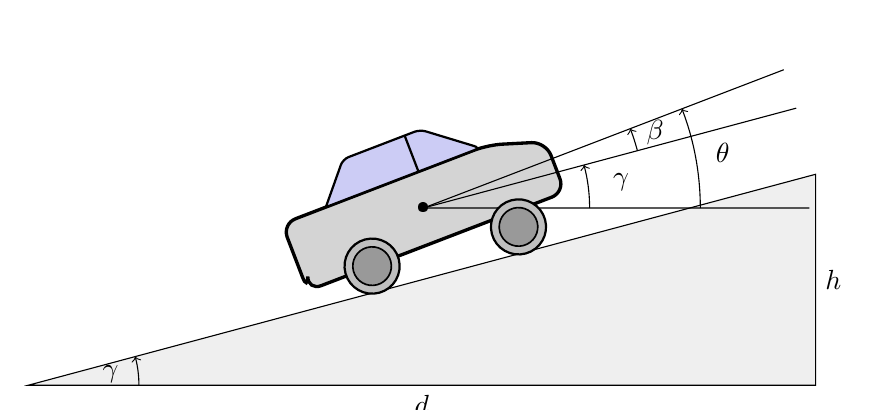
\begin{tikzpicture}[scale=1]
    % Define/Calc ramp parameters
    % Ramp length
    \def\rl{10};
    % Ramp angle [deg]
    \def\ra{15};
    % Ramp height
    \def\rh{{tan(\ra)*\rl}};

    % RAMP
    % Define the points
    \coordinate (A) at (0,0);
    \coordinate (B) at ($(A) + (\rl,0)$);
    \coordinate (C) at ($(B) + (0,\rh)$);
    % Draw and fill ramp
    \filldraw[draw=black, fill=lightgray!25] (A) -- (B) -- (C) -- cycle;
    % Label length and draw angle
    \path (A) -- (B) node [midway, below] {$d$}
    pic[draw, ->, angle radius=40pt,
            angle eccentricity=0.75, "$\gamma$"]{angle=B--A--C};
    % Label height
    \draw (B) -- (C) node [midway, right] {$h$};

    % CAR
    % Tilt whole car
    \begin{scope}[scale=0.7, xshift=\rl*0.5 cm, yshift=1.9 cm, rotate=\ra]

        % Car height
        \def\ch{2}
        % Car length
        \def\cl{5}
        % Car body height
        \def\bh{\ch*0.65}
        % Roof length
        \def\rl{\cl*0.6}
        % Roof height
        \def\rh{\ch*0.35}
        % Car tilt angle
        \def\ct{6}

        % Tilt body without wheels
        \begin{scope}[rotate=\ct, yshift=-0.2cm]
            % Anchor point is southwest
            \coordinate (b) at (0,0);
            % Offset to roof and wheels
            \coordinate (r) at ($(b) +(\cl*0.17,\ch*0.65)$);
            \coordinate (w) at ($(b) + (\cl*0.25,0)$);
            % Body
            \draw[black, fill=black!17, rounded corners=1.2ex, very thick]
            (b) -- ++(0,\bh) -- ++(\cl*1/5,0) --  ++(\cl*3/5,0) -- ++(\cl*1/5,-\bh*0.25)
            -- ++(0, -\bh*0.75) -- (b) -- cycle;
            % Roof
            \draw[very thick, rounded corners=0.5ex, fill=black!20!blue!20!white,thick]
            (r) -- ++(0.2*\rl,\rh) -- ++(0.5*\rl,0) -- ++(0.3*\rl,-\rh) -- (r);
            \draw[thick] (r)++(\rl*0.6,0) -- ++(0,\rh);

            % Car middle point
            \coordinate (m) at (\cl*0.5, \bh*0.5);
            \node at (m) {\textbullet};
            % Line parallel to body
            \draw (m) -- ++(7,0) coordinate (pb);
            % Line parallel to ramp
            \draw[rotate = -\ct] (m) -- ++(7,0) coordinate (pr);
            % Line parallel to ground
            \draw[rotate = -\ct-\ra] (m) -- ++(7,0) coordinate (pg);
            % Draw angles
            \path (pb) -- (pr)
            pic[draw, ->, angle radius=60pt, angle eccentricity=1.2, "$\gamma$"] {angle = pg--m--pr}
            pic[draw, ->, angle radius=80pt, angle eccentricity=1.1, "$\beta$"] {angle = pr--m--pb}
            pic[draw, ->, angle radius=100pt, angle eccentricity=1.1, "$\theta$"] {angle = pg--m--pb};
        \end{scope}

        % Wheels
        \draw[draw=black,fill=gray!50,thick] (w) circle (.5);
        \draw[draw=black,fill=gray!50,thick] (w) ++(\cl*0.55,0) circle (.5);
        % Inner wheels
        \draw[draw=black,fill=gray!80,semithick] (w) circle (.35);
        \draw[draw=black,fill=gray!80,semithick] (w) ++(\cl*0.55,0) circle (.35);
    \end{scope}
\end{tikzpicture}
\end{document}
	\caption[Ramp angle definition]{Car driving on a ramp. Due to forward acceleration the car tilts back.}
	\label{fig:tikz_car_tilt}
\end{figure}
The road grade $\alpha$ is the angle between the road plane and the ground plane.
The ground plane is perpendicular to the gravity vector.
The road grade can be represented as an angle
\begin{equation}
	\alpha = \arctan(\frac{h}{d})
\end{equation}
or in percentage
\begin{equation}
	r = 100\cdot\tan(\alpha).
\end{equation}
The pitch angle $\theta$ of the car is defined as the angle between the ground plane and the longitudinal axis of the car.
If the car accelerates or decelerates the suspension does get compressed in the back or respectively front, which makes the pitch angle not in alignment with the road grade anymore.
The difference between the two angles is defined as $\beta = \theta - \alpha$ and may also occur due to rotational movement or vibrations.
The mentioned variables are visualized in \cref{fig:tikz_car_tilt}.



\section{Coordinate frames}
\label{sec:coordinate_frames}
A common problem is that the coordinate frames of the sensors are usually not aligned with the device (in this case the car) frame, see \cref{fig:tikz_car_frames}.
To get meaningful results, the sensor frames must first be aligned with the car frame.
Semi-automatic calibration methods for the \gls{imu} and \gls{lidar} sensor will be represented in \cref{ssec:calibration_imu} and \cref{ssec:calibration_lidar} respectively, which determine the necessary rotation to align both frames.
But the translation difference between the coordinate frames can not be easily estimated or requires a more sophisticated calibration setup which was not available, and must be measured by hand.\\
The coordinate frame of the car has the x-axis pointing in the direction of travel , the y-axis to the left and the z-axis upwards.
The center of the coordinate system of the car is located at the center in the front of the car at the height of the wheel axle.
\begin{figure}[htb]
	\centering
	\documentclass[11pt]{standalone}
\usepackage{tikz}
\usetikzlibrary{angles, calc, decorations.pathmorphing, quotes, spy}

\begin{document}
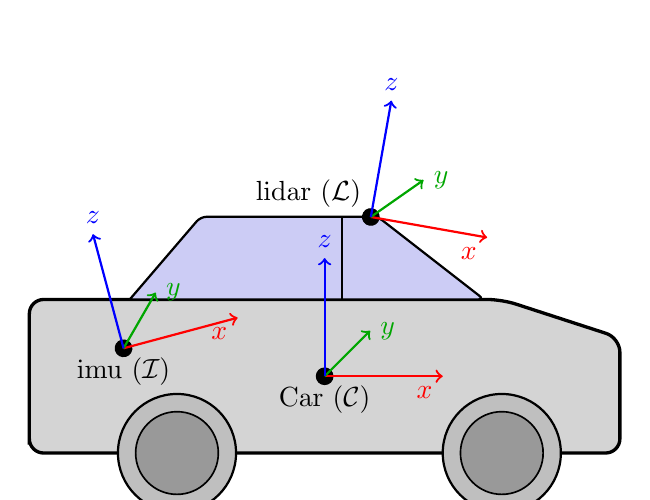
\begin{tikzpicture}[scale=1.5]
    % Define car parameters
    % Car height
    \def\ch{2}
    % Car length
    \def\cl{5}
    % Car body height
    \def\bh{\ch*0.65}
    % Roof length
    \def\rl{\cl*0.6}
    % Roof height
    \def\rh{\ch*0.35}
    % Car tilt angle
    \def\ct{6}
    % Anchor point is southwest
    \coordinate (b) at (0,0);
    % Offset to roof and wheels
    \coordinate (r) at ($(b) +(\cl*0.17,\ch*0.65)$);
    \coordinate (w) at ($(b) + (\cl*0.25,0)$);

    % Body
    \draw[black, fill=black!17, rounded corners=1.2ex, very thick]
    (b) -- ++(0,\bh) -- ++(\cl*1/5,0) --  ++(\cl*3/5,0) -- ++(\cl*1/5,-\bh*0.25)
    -- ++(0, -\bh*0.75) -- (b) -- cycle;
    % Roof
    \draw[very thick, rounded corners=0.5ex, fill=black!20!blue!20!white,thick]
    (r) -- ++(0.2*\rl,\rh) -- ++(0.5*\rl,0) -- ++(0.3*\rl,-\rh) -- (r);
    % \draw[thick] ($(r) + (\cl*0.5,\bh)$) -- ++(0,\rh);
    \draw[thick] (r)++(\rl*0.6,0) -- ++(0,\rh);

    % Wheels
    \draw[draw=black,fill=gray!50,thick] (w) circle (.5);
    \draw[draw=black,fill=gray!50,thick] (w) ++(\cl*0.55,0) circle (.5);
    % Inner wheels
    \draw[draw=black,fill=gray!80,semithick] (w) circle (.35);
    \draw[draw=black,fill=gray!80,semithick] (w) ++(\cl*0.55,0) circle (.35);

    % Car middle point
    \coordinate (m) at (\cl*0.5, \bh*0.5);
    \filldraw (m) circle (2pt) node[below] {Car ($\mathcal{C}$)};
    % Coordinate frames
    \draw[thick,->, red] (m) -- ++(1,0,0) node[anchor=north east]{$x$};
    \draw[thick,->, black!35!green] (m) -- ++(0,0,-1) node[anchor=west]{$y$};
    \draw[thick,->, blue] (m) -- ++(0,1,0) node[anchor=south]{$z$};

    % IMU middle point (random)
    \begin{scope}[rotate=15]
        \coordinate (mi) at (\cl*0.2, \bh*0.5);
        \filldraw (mi) circle (2pt) node[below] {\gls{imu} ($\mathcal{I}$)};
        % Coordinate frames
        \draw[thick,->, red] (mi) -- ++(1,0,0) node[anchor=north east]{$x$};
        \draw[thick,->, black!35!green] (mi) -- ++(0,0,-1) node[anchor=west]{$y$};
        \draw[thick,->, blue] (mi) -- ++(0,1,0) node[anchor=south]{$z$};
    \end{scope}

    % LIDAR middle point (random)
    \begin{scope}[rotate=-10]
        \coordinate (ml) at (2.5, 2.47);
        \filldraw (ml) circle (2pt) node[above left] {\gls{lidar} ($\mathcal{L}$)};
        % Coordinate frames
        \draw[thick,->, red] (ml) -- ++(1,0,0) node[anchor=north east]{$x$};
        \draw[thick,->, black!35!green] (ml) -- ++(0,0,-1) node[anchor=west]{$y$};
        \draw[thick,->, blue] (ml) -- ++(0,1,0) node[anchor=south]{$z$};
    \end{scope}
\end{tikzpicture}
\end{document}
	\caption[Sensor coordinate frames]{Example of a typical sensor setup. All measurements of the sensors must be transformed, such that they align with the car frame.}
	\label{fig:tikz_car_frames}
\end{figure}



\section{\glsentryshort{imu}}
\label{sec:methods_imu}
Before being able to apply the different methods, a transformation from the sensor frame to the car frame is necessary.
This is described in \cref{ssec:calibration_imu}.
After the transformation an estimation of the car's pitch angle is possible, for which different methods are presented in \cref{ssec:road_grade_estimation}.
In \cref{ssec:ramp_detection_imu} a ramp detection algorithm based on the estimated pitch angle is presented.
Furthermore, a method to estimate the average ramp angle and length of the ramp is proposed.


\subsection{Calibration}
\label{ssec:calibration_imu}
\begin{figure}[htb]
	\centering
	\begin{subfigure}[b]{0.3\textwidth}
		\centering
		\documentclass[11pt]{standalone}
\usepackage{tikz}

\newcommand{\rotateRPY}[3]% roll, pitch, yaw
{   \pgfmathsetmacro{\rollangle}{#1}
    \pgfmathsetmacro{\pitchangle}{#2}
    \pgfmathsetmacro{\yawangle}{#3}

    % to what vector is the x unit vector transformed, and which 2D vector is this?
    \pgfmathsetmacro{\newxx}{cos(\yawangle)*cos(\pitchangle)}
    \pgfmathsetmacro{\newxy}{sin(\yawangle)*cos(\pitchangle)}
    \pgfmathsetmacro{\newxz}{-sin(\pitchangle)}
    \path (\newxx,\newxy,\newxz);
    \pgfgetlastxy{\nxx}{\nxy};

    % to what vector is the y unit vector transformed, and which 2D vector is this?
    \pgfmathsetmacro{\newyx}{cos(\yawangle)*sin(\pitchangle)*sin(\rollangle)-sin(\yawangle)*cos(\rollangle)}
    \pgfmathsetmacro{\newyy}{sin(\yawangle)*sin(\pitchangle)*sin(\rollangle)+ cos(\yawangle)*cos(\rollangle)}
    \pgfmathsetmacro{\newyz}{cos(\pitchangle)*sin(\rollangle)}
    \path (\newyx,\newyy,\newyz);
    \pgfgetlastxy{\nyx}{\nyy};

    % to what vector is the z unit vector transformed, and which 2D vector is this?
    \pgfmathsetmacro{\newzx}{cos(\yawangle)*sin(\pitchangle)*cos(\rollangle)+ sin(\yawangle)*sin(\rollangle)}
    \pgfmathsetmacro{\newzy}{sin(\yawangle)*sin(\pitchangle)*cos(\rollangle)-cos(\yawangle)*sin(\rollangle)}
    \pgfmathsetmacro{\newzz}{cos(\pitchangle)*cos(\rollangle)}
    \path (\newzx,\newzy,\newzz);
    \pgfgetlastxy{\nzx}{\nzy};
}
\tikzset{RPY/.style={x={(\nxx,\nxy)},y={(\nyx,\nyy)},z={(\nzx,\nzy)}}}
% NOTE: I changed y and z axes, so it is now RYP instead of RPY

\begin{document}
\begin{tikzpicture}
    \draw[-latex] node at (3.5,0,0) {x} (0,0,0) -- (3,0,0);
    \draw[-latex] node at (0,0,-3.5) {y} (0,0,0) -- (0,0,-3);
    \draw[-latex] node at (0,3.5,0) {z} (0,0,0) -- (0,3,0);

    \rotateRPY{5}{5}{20}
    \begin{scope}[draw=red, text=red,fill=red,densely dashed,RPY]
        \draw[-latex] node at (3.5,0,0) {x} (0,0,0) -- (3,0,0);
        \draw[-latex] node at (0,0,-3.5) {y} (0,0,0) -- (0,0,-3);
        \draw[-latex] node at (0,3.5,0) {z} (0,0,0) -- (0,3,0);
    \end{scope}
    % \node[fill=white,fill opacity=0.7,text opacity=1] {RPY: $r$,$p$,$y$};
\end{tikzpicture}
\end{document}
		\caption{No axes are aligned}
		\label{fig:tikz_frame_transformation_init}
	\end{subfigure}
	\hfill
	\begin{subfigure}[b]{0.3\textwidth}
		\centering
		\input{Graphics/TikZ/frame_transformation_intermediate.tex}
		\caption{Z axes are aligned}
		\label{fig:tikz_frame_transformation_intermediate}
	\end{subfigure}
	\hfill
	\begin{subfigure}[b]{0.3\textwidth}
		\centering
		\input{Graphics/TikZ/frame_transformation_final.tex}
		\caption{All axes are aligned}
		\label{fig:tikz_frame_transformation_final}
	\end{subfigure}
	\caption[Frame transformation]{Frame transformation from the \gls{imu} frame \textcolor{red}{$\mathcal{I}$}, over the intermediate frame \textcolor{blue}{$\mathcal{B}$} to the car frame \textcolor{green}{$\mathcal{C}$}.}
	\label{fig:tikz_frame_transformation}
\end{figure}
The \gls{imu} is usually not placed in such a way, that the coordinate frame of the device $\mathcal{I}$ aligns with that of the car $\mathcal{C}$, see \cref{fig:tikz_frame_transformation_init}.
Because of that, a transformation between the two frames must be found.
This can be achieved using a rotation matrix \mtf{i}{c} $\in \mathbb{R}^{3\times3}$ which transforms the measurements of the linear acceleration $\vincs{a}{I}_n \in \mathbb{R}^{1\times3}$ and angular velocity ${\vincs{v}{I}_n \in \mathbb{R}^{1\times3}}$ into the car frame.
Note that the upper index to the left of the matrix symbol denotes the source frame, whereas the destination frame is written below it.
$n \in \mathbb{N}$ is the time step.\\
During standstill, the only measurable acceleration besides noise and bias is the acceleration due to gravity.
Assuming the car stands on flat ground, the gravity acceleration in the car frame is measured only in upwards z-direction.
Using this, a transformation from \gls{imu} frame $\mathcal{I}$ to the intermediate frame $\mathcal{B}$ can be found.
In the new $\mathcal{B}$ frame both z-axes are aligned $\vincs{z}{b} = \vincs{z}{c}$ and thus the pitch and roll angle between the two frames become zero.
Note that this is not necessarily true for the other axes, $\vincs{x}{b}\neq\vincs{x}{c}$ and $\vincs{y}{b}\neq\vincs{y}{c}$, see \cref{fig:tikz_frame_transformation_intermediate}.\\
According to Euler's rotation theorem, which says that any arbitrary rotation of a rigid body while holding one point (origin) fixed can be achieved by a rotation around a single fixed axis passing through the origin, there exists one rotation axis $\mathbf{j}$ and rotation angle $\alpha$ to achieve this.\\
As described in \cref{subsec:vector_projection}, the rotation axis needed for the transformation can be calculated by
\begin{equation}
	\vb{j} = \frac{\vincs{\vu{a}}{i} \cp \vincs{\vu{z}}{c}}{\norm{\vincs{\vu{a}}{i} \cp \vincs{\vu{z}}{c}}}
\end{equation}
and the rotation angle with
\begin{equation}
	\alpha = \arccos(\vincs{\vu{a}}{i}\vdot \vincs{\vu{z}}{c})
\end{equation}
with $\vincs{\vu{a}}{i} \in \mathbb{R}^{1\times3}$ being the normalized measured linear acceleration in the \gls{imu} frame and \vincs{\vu{z}}{c} the (normalized) z-axis of the car.\\
The quaternion
\begin{equation}
	\qtf{i}{b} =
	\begin{bmatrix}
		\vb{j}\vdot\sin(\frac{\alpha}{2}) \\
		\cos(\frac{\alpha}{2})
	\end{bmatrix}
\end{equation}
then describes the rotation between the two frames.\\
Now that the z-axes of the $\mathcal{I}$ and $\mathcal{C}$ frame are aligned, the x- and y-axis can be aligned by a rotation $\beta$ around the z-axis.
This yaw correction could usually be achieved using the magnetometer measurements, but because those are heavily obscured indoors and especially in the parking garage \cite{Li2012}, another solution must be found.
A possible solution to this problem is accelerating the car straightforward and then using the accelerometer to measure along which axis the acceleration occurred.
Assuming the car tilt (pitch) during the acceleration is minimal, the acceleration is only being measured along the x- and y-axis.
The resulting vector is being aligned with the forward axis of the car, such that $\vincs{\hat{a}}{b} = \vincs{x}{c}$, in the same way as before.
Resulting in the rotation angle
\begin{equation}
	\beta = \arccos(\vincs{\vu{a}}{b} \vdot \vincs{\hat{x}}{c})
\end{equation}
and the quaternion
\begin{equation}
	\qtf{b}{c} =
	\begin{bmatrix}
		\vincs{\hat{z}}{c}\vdot\sin(\frac{\beta}{2}) \\
		\cos(\frac{\beta}{2})
	\end{bmatrix}.
\end{equation}
The two quaternions can then be concatenated (in reverse order) to get the final quaternion
\begin{equation}
	\qtf{i}{c} = \qtf{b}{c} \otimes  \qtf{i}{b}
\end{equation}
which transforms the measurements of the \gls{imu} to the car frame.\\
The quaternion is then converted into a rotation matrix using \cref{eq:q_to_M}, because it reduces the computation time.
The measurements $\mathbf{A}$ can be transformed using
\begin{equation}
	\vincs{A}{c} = \mtf{i}{c} \vdot \vincs{A}{i}.
\end{equation}


\subsection{Road grade estimation}
\label{ssec:road_grade_estimation}
\subsubsection{Accelerometer}
\label{ssec:linear_acceleration_only}
If the car stands still, the only measurable acceleration besides measurement errors is the acceleration due to gravity.
When standing on flat ground, only the z-axis measures an acceleration.
But when the car is tilted, e.g. on a ramp, the gravity is measured also by the x-axis (which points forward), see \cref{fig:tikz_car_gravity}.
The proportion of the acceleration measured along the x-axis $\vb{a}_\mathrm{x} $ of the overall gravity $\vb{g}$ can then be used to determine the pitch angle in the following way
\begin{equation}
	\label{eq:ang_from_acc}
	\theta_\mathrm{acc}  = \arcsin(\frac{\vb{a}_x}{\norm{\vb{g}}})
\end{equation}
with $\norm{\vb{g}}$ being the magnitude of the overall measured acceleration.
According to the definition, the angle is zero if the car is parallel to the ground and \SI{90}{\degree} if the front of the car would be pointing straight up.
The angle is positive when driving up a ramp and negative if driving down.\\
Disadvantages of this method are that the acceleration measurements are quite noisy and that no other accelerations are taken into account, e.g. the on track acceleration $\vb{a}_\mathrm{at}$ caused by the motor.
This is a problem when the car has a non-zero acceleration, because the acceleration measured by the \gls{imu} along the x-axis is given by
\begin{equation}
	\vb{a}_\mathrm{x} = \vb{a}_\mathrm{at} + \vb{g}_\mathrm{x}
\end{equation}
and $\vb{a}_\mathrm{x} = \vb{g}_\mathrm{x} $ only holds true, when the car is driving with constant velocity or standing still.
A better approach, which incorporates the accelerations caused by the car, is described in \cref{subsubsec:gravity_method}.
\begin{figure}[htpb]
	\centering
	\documentclass[11pt]{standalone}
\usepackage{tikz}
\usetikzlibrary{angles, calc, decorations.pathmorphing, quotes, spy}

\begin{document}
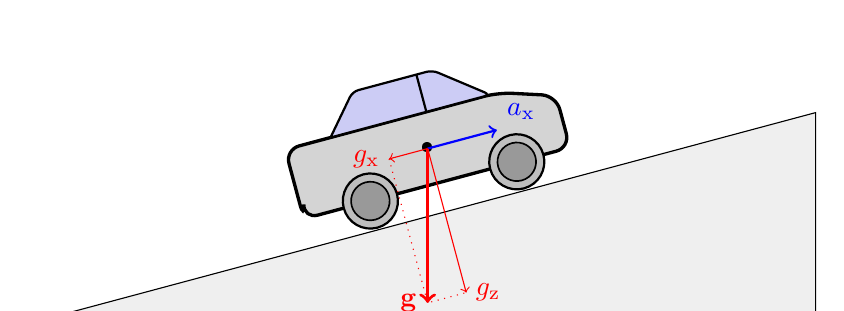
\begin{tikzpicture}[scale=1]
    % Define/Calc ramp parameters
    % Ramp length
    \def\rl{10};
    % Ramp angle [deg]
    \def\ra{15};
    % Ramp height
    \def\rh{{tan(\ra)*\rl}};

    % RAMP
    % Define the points
    \coordinate (A) at (0,0);
    \coordinate (B) at ($(A) + (\rl,0)$);
    \coordinate (C) at ($(B) + (0,\rh)$);
    % Draw and fill ramp
    \filldraw[draw=black, fill=lightgray!25] (A) -- (B) -- (C) -- cycle;

    % CAR
    % Tilt whole car
    \begin{scope}[scale=0.7, xshift=\rl*0.5 cm, yshift=1.9 cm, rotate=\ra]
        % Car height
        \def\ch{2}
        % Car length
        \def\cl{5}
        % Car body height
        \def\bh{\ch*0.65}
        % Roof length
        \def\rl{\cl*0.6}
        % Roof height
        \def\rh{\ch*0.35}
        % Car tilt angle
        \def\ct{6}

        % Anchor point is southwest
        \coordinate (b) at (0,0);
        % Offset to roof and wheels
        \coordinate (r) at ($(b) +(\cl*0.17,\ch*0.65)$);
        \coordinate (w) at ($(b) + (\cl*0.25,0)$);
        % Body
        \draw[black, fill=black!17, rounded corners=1.2ex, very thick]
        (b) -- ++(0,\bh) -- ++(\cl*1/5,0) --  ++(\cl*3/5,0) -- ++(\cl*1/5,-\bh*0.25)
        -- ++(0, -\bh*0.75) -- (b) -- cycle;
        % Roof
        \draw[very thick, rounded corners=0.5ex, fill=black!20!blue!20!white,thick]
        (r) -- ++(0.2*\rl,\rh) -- ++(0.5*\rl,0) -- ++(0.3*\rl,-\rh) -- (r);
        \draw[thick] (r)++(\rl*0.6,0) -- ++(0,\rh);

        % % Car middle point
        \coordinate (m) at (\cl*0.5, \bh*0.5);
        \node at (m) {\textbullet};
        % Wheels
        \draw[draw=black,fill=gray!50,thick] (w) circle (.5);
        \draw[draw=black,fill=gray!50,thick] (w) ++(\cl*0.55,0) circle (.5);
        % Inner wheels
        \draw[draw=black,fill=gray!80,semithick] (w) circle (.35);
        \draw[draw=black,fill=gray!80,semithick] (w) ++(\cl*0.55,0) circle (.35);

        % Draw car acceleration
        \draw[blue, thick, ->] (m) -- ++(1.3,0) node[anchor=south west]{$a_\mathrm{x}$};
        % Gravity vectors
        % Length of g vector
        \def\gl{2.8}
        % Length of g vector components
        \def\gxl{{\gl*sin(\ra)}}
        \def\gzl{{\gl*cos(\ra)}}
        % Draw vectors
        \draw[red, ->, very thick, rotate=-\ra] (m) -- ++(0,-\gl) node[anchor=east](g_end){$\mathbf{g}$};
        \draw[red, thin, ->] (m) -- ++(-\gxl,0) node[anchor=east]{$g_\mathrm{x}$};
        \draw[red, thin, ->] (m) -- ++(0,-\gzl) node[anchor=west]{$g_\mathrm{z}$};
        \draw[red, dotted] ($(m)+(-\gxl,0)$) -- ++(0,-\gzl) -- ++(\gxl,0);
        % \draw[red, dotted] ($(m)+(0,0)$) -- ++(0,-\gzl) -- ++(\gxl,0);
    \end{scope}
\end{tikzpicture}
\end{document}
	\caption{The prevailing accelerations when a car is accelerating on a ramp.}
	\label{fig:tikz_car_gravity}
\end{figure}
\subsubsection{Gyroscope}
\iimprov{Find good source and use it as a guide}
The gyroscope measures the angular velocity, which must be integrated with respect to time, to get a rotation angle.
The angular velocity the rate of change of an angle and is defined as
\begin{equation}
	% \boldsymbol{\omega}  = \frac{\Delta\theta}{\Delta t}
	\boldsymbol{\omega}  =  \dv{\boldsymbol{\theta}}{t}.
\end{equation}
Assuming that the measurements of the gyroscope are continuous in time, the current angle $\boldsymbol{\theta}(t)$ at time $T$ can be computed with the integral
\begin{equation}
	\boldsymbol{\theta}(t) = \boldsymbol{\theta}_0 + \int_0^T \boldsymbol{\omega}(t)\dd{t}
\end{equation}
with $\boldsymbol{\theta}_0$ being the initial angle.\\
In practice, however, the \gls{imu} provides samples at discrete times $k$ and $k-1$.
Assuming that the signal remains constant during the time $\Delta t$ between the two samples, the integral can be numerical approximated.
An error will be introduced by the approximation, but it will be small if the sample rate is sufficiently high.
Different techniques exist, using the ? method the new angle after a change between two samples can be calculated with
\begin{equation}
	\boldsymbol{\theta}_k = \boldsymbol{\theta}_\mathrm{k - 1} + \boldsymbol{\omega}_k\Delta t.
\end{equation}
Similarly, the angle based on multiple consecutive measurements can be calculated by the sum of all previous measurements
\begin{equation}
	\label{eq:ang_from_gyro}
	\boldsymbol{\theta}_k = \boldsymbol{\theta}_0 + \sum_{i = 1}^k \boldsymbol{\omega}_i \Delta t
\end{equation}
with $\boldsymbol{\theta}_0$ being the initial angle at the start of the measurement, which must be known beforehand.\\
To get the pitch angle $\theta_\mathrm{gyr}$, only the measurements along the y-axis are of interest (see \cref{fig:tikz_car_frames}).
The pitch angle at time $k$ is given by
\begin{equation}
	\theta_\mathrm{k, gyr} = \theta_{0, \mathrm{gyr} } + \sum_{i = 1}^{k} \boldsymbol{\omega}_\mathrm{i, y} \Delta t.
\end{equation}
Disadvantages of using only the angular velocity are that the estimations are not reliable over a long period of time.
The random walk introduced by integrating white noise or a constant bias causes the estimation to drift away from the true value.


\subsubsection{Complementary filter}
The complementary uses both the linear acceleration and angular velocity measurements and combines them using sensor fusion, such that the good properties of each sensor are used to reduce the poor properties of the other.
The angle estimation obtained from the linear acceleration measurements is reliable in the long-term, but is quite noisy.
The estimation from the angular velocity measurements on the other hand provide good short-term accuracy, but should not be used for longer estimations due to drift.\\
These properties can be interpreted in the frequency domain.
The error from the accelerometer data is subject to high frequency noise, whereas the estimation error from the gyroscope is mostly due to low frequency noise \cite{2007Colton}.
To minimize the error of the linear acceleration estimate, a \gls{lpf} should be used.
A \gls{lpf} passes all signals with frequency lower than a certain cut-off frequency $f_0$ and attenuates signals with a frequency above $f_0$.
In contrast, a \gls{hpf} should be used on the estimate of the gyroscope.
A \gls{hpf} works exactly opposite to a \gls{lpf}.
It blocks signals with a frequency below $f_0$ while allowing signals over this frequency to pass through \cite{Lyons1996}. A block diagram of the complementary filter is shown in \cref{fig:tikz_complementary_filter}.\\
\begin{figure}[htb]
	\centering
	\documentclass[11pt]{standalone}
\usepackage{tikz}
\usepackage{physics}

\usetikzlibrary{calc, positioning}

\begin{document}
% Define styles
\tikzstyle{block} = [draw, minimum width=2cm, minimum height=1.2cm]

\begin{tikzpicture}
    % Sum shape
    \node[draw, circle, minimum size=0.6cm] (sum) at (0,0){+};

    % LP-Filter block
    \node [block, above left=0.1cm and 1cm of sum] (lpf) {Low-Pass Filter};
    % HP-Filter block
    \node [block, below left=0.1cm and 1cm of sum] (hpf) {High-Pass Filter};
    % Integrator block
    \node [draw, minimum height=1.2cm, left=1.5cm of lpf] (acc) {$\arcsin(\frac{\vb{a}_x}{\norm{\vb{g}}})$};
    \node [draw, minimum height=1.2cm, left=2.25cm of hpf] (int) {$\int$};

    % Connect blocks with sum
    \draw[-stealth] (lpf.east) -| (sum.north);
    \draw[-stealth] (hpf.east) -| (sum.south);

    % Input signals
    \node [left=5cm of lpf] (start_acc){};
    \node [below=1.7cm of start_acc] (start_gyr){};
    \draw[stealth-] (acc.west) -- (start_acc) node[left]{$\vb{a}$};
    \draw[-stealth] (acc.east) -- (lpf.west) node[midway, above]{$\theta_\mathrm{acc}$};
    \draw[stealth-] (int.west) -- (start_gyr) node[left]{$\boldsymbol{\omega}$};
    \draw[-stealth] (int.east) -- (hpf.west) node[midway, above]{$\theta_\mathrm{gyr}$};
    \draw[-stealth] (sum.east) -- ++(1,0) node[right]{$\hat{\theta}$};
\end{tikzpicture}
\end{document}
	\caption{Block diagram of the complementary filter}
	\label{fig:tikz_complementary_filter}
\end{figure}
The angle estimation obtained from the linear acceleration (\cref{eq:ang_from_acc}) will be referred to as $\theta_\mathrm{acc}$, the angle estimation from the gyroscope estimation as $\theta_\mathrm{gyr}$ and the fused estimation of the complementary filter will be denoted as $\hat{\theta}$.
As seen in \cref{eq:ang_from_gyro}, $\theta_\mathrm{gyr}$ is calculated by integrating the angular velocity $\omega_\mathrm{gyr} $ measured by the gyroscope.
The Laplace transformation can be used to transform the angles from the time domain to the frequency domain.
The angles $\theta_\mathrm{acc}$, $\theta_\mathrm{gyr}$ and $\hat{\theta}$ will be denoted as $\Theta_\mathrm{acc}(s)$, $\Theta_\mathrm{gyr}(s)$ and $\hat{\Theta}(s)$ in the frequency domain, the gyroscope measurements $\omega_\mathrm{gyr} $ as $\Omega_\mathrm{gyr} (s)$.
The complimentary filter estimate is computed by
\begin{align}
	\label{eq:compl_filter_laplace}
	\hat{\Theta}(s) & = G_\mathrm{low}(s)\Theta_\mathrm{acc}(s) + (1 - G_\mathrm{low}(s))\Theta_\mathrm{gyr}(s) \nonumber   \\
	                & = G_\mathrm{low}(s)\Theta_\mathrm{acc}(s) + (1 - G_\mathrm{low}(s))\frac{1}{s}\Omega_\mathrm{gyr} (s)
\end{align}
where $G_\mathrm{low}(s)$ is the transfer function of a \gls{lpf} and $1-G_\mathrm{low}(s) = G_\mathrm{high}(s)$ the of a \gls{hpf} \cite{Kok2017}.
The sum of $G_\mathrm{low}(s)$ and $1-G_\mathrm{low}(s)$ is equal to one, which means that the cut-off frequency of both filters must be the same.
The transfer functions are defined as
\begin{equation}
	\label{eq:lpf}
	G_\mathrm{low} (s) = \frac{1}{1 + \alpha s}
\end{equation}
for the \gls{lpf} and
\begin{equation}
	\label{eq:hpf}
	G_\mathrm{high} (s) = \frac{\alpha s}{1 + \alpha s}
\end{equation}
for the \gls{hpf}, when using a first-order filter.
$\alpha$ is the filter coefficient and is depended on the cut-off frequency in the following way
\begin{equation}
	\alpha
	= \frac{\tau}{\tau + T}
	% = \frac{1}{w_0}
	= \frac{1}{2\pi f_0}
	\label{eq:filter_f0}
\end{equation}
with $\tau$ being the time constant of the filter and $T$ being the sample period.
Inserting \cref{eq:lpf} and \cref{eq:hpf} in \cref{eq:compl_filter_laplace} and using inverse Laplace transformation as well as Euler backward discretization, the complementary filter can be written in discrete time as
\begin{equation}
	\hat{\theta}_k = \gamma\left(\hat{\theta}_{k - 1} + T \omega_{k, \mathrm{gyr}}\right) + (1 - \gamma) \theta_{k, \mathrm{acc}},
\end{equation}
with
\begin{equation}
	\label{eq:filter_gain}
	\gamma = \frac{\alpha}{\alpha + T} \in [0,1]
\end{equation}
being the filter gain.
The choice of the parameter $\alpha$ (and hence $\gamma$) determines, how much each of the two measurements should be trusted.
Selecting a small $\alpha$ ($\gamma$ close to zero) results in a high cut-off frequency.
The estimation then mostly uses the accelerometer data.
Contrary, a high value of $\alpha$ leads to a $\gamma$ close to one and low cut-off frequency, where the gyroscope estimation is trusted more \cite{1997Baerveldt}.\\
% A decrease of $\alpha$ leads to a smoother signal, but at the cost of adding some additional time delay.
Selecting the right filter coefficient is a known problem and is usually solved by calculating an initial guess followed by fine-tuning by hand to get the desired result.
One option to get an initial guess is by measuring the drift of the gyroscope and selecting the filter coefficient accordingly.
The time $T_\mathrm{free}$ where the drift of the angle estimation from the gyroscope is negligible, is inversely proportional to the cut-off frequency $f_0 = \frac{1}{T_\mathrm{free}}$.
E.g. if the drift from the gyroscope is only negligible for \SI{10}{\second} then the cut-off frequency should be chosen at $f_0 = \frac{1}{\SI{10}{\second}} = \SI{0.1}{\hertz}$ or higher.
The filter gain can then be calculated using \cref{eq:filter_f0} and \cref{eq:filter_gain}.
Using the previous example and assuming a sample frequency of \SI{100}{\hertz}, the filter gain would then be $\gamma = 0.9938$.
For the experiment a cut-off frequency of $f_0=?$ was chosen, resulting in a filter coefficient of $\alpha = ?$ and a filter gain of $\gamma = ?$.

\subsubsection{Gravity method}
\label{subsubsec:gravity_method}
% \subsubsubsection{Car acceleration from odometer data}
% \label{subsubsec:acc_from_odom}
As described in \cref{ssec:linear_acceleration_only}, the linear acceleration measurements can be used to determine the pitch angle.
But the estimation is only valid under the condition, that there are no accelerations other than the acceleration due to gravity.
This condition is not necessarily true when the car is driving, during which the car can accelerate or brake.
To get the correct estimation, the car's acceleration must be subtracted from the measurement.
\paragraph{Car acceleration from odometer data}\mbox{}\\
Using the wheel speed measurements the velocity of the vehicle can be calculated.
Because the wheel speed sensors only deliver the speed of each wheel, a model has to be used to estimate the velocity of the car.
Because setting one wheel speed measurement equal to the velocity of the car would lead to a wrong estimation, since during turns the left and right wheels travel at different speeds, the wheel on the inner side of the turn travels slower, than the outer wheel.
A simple yet sufficiently accurate model to calculate the car velocity from the wheel speeds is the linear single track model \cite{Mitschke2014}.
In this model both wheels on one axis are replaced with one wheel in the middle.
The linear assumption holds true for low lateral accelerations (up to \SI{4}{\metre\per\second}), which will not be surpassed in the experiments.
Using the assumptions from above, the car velocity $v_\mathrm{car}(t)$ can be calculated by
\begin{align}
	\alpha(t)         & = \frac{v_\mathrm{rl}(t) - v_\mathrm{rr}(t)}{d}                  \\
	\gamma(t)         & = \frac{\alpha(t)}{f_\mathrm{odom}}                              \\
	v_\mathrm{car}(t) & = \frac{v_\mathrm{rl}(t) + v_\mathrm{rr}(t)}{2}\cdot\cos(\gamma)
	\label{eq:v_car}
\end{align}
with $v_\mathrm{rl} \text{ and } v_\mathrm{rr}$ being the wheel speeds of the rear right and rear left wheel respectively, $d$ the track width and $\gamma$ is the yaw angle of the car, which can be calculated from the steering wheel angle.\\
To calculate the acceleration of the vehicle, the first derivative of the velocity must be taken, using
\begin{equation}
	a_\mathrm{car}(t) = \dv{t}v_\mathrm{car}(t).
\end{equation}
But because all measurements are discrete, numerical differentiation is necessary, it can be approximated using the backward difference
\begin{equation}
	a_\mathrm{k, car} = \frac{v_\mathrm{k, car} - v_\mathrm{k - 1, car}}{T}
\end{equation}
with $T$ being the step size, which is equal to the rate of the sensor.\\
Because the from the wheel speed sensors calculated velocity is discrete in time, quantized and not free of noise, a simple derivation would amplify the noise.
Hence, the measurements must first be filtered.
\itodo{Investigate other filters such as savitzky-golay once and for all}
A very simple solution is to use a moving average filter, which is a simple average of the last $N$ measurements.
The finite difference of the approximation can then be calculated.
\paragraph{Gravity method}\mbox{}\\
The prevailing accelerations during a positive acceleration can be seen in \cref{fig:tikz_car_gravity}.
When the car brakes, the direction of $\vb{a}_\mathrm{x}$ inverts.
The car pitch angle calculation is the same as in \cref{eq:ang_from_acc}, just that now the car acceleration $\vb{a}_\mathrm{at}$ is taken into account.
\begin{equation}
	\label{eq:ang_from_acc_gravity}
	\alpha = \arcsin\left(\frac{\vb{a}_\mathrm{x} - \vb{a}_\mathrm{at}}{\norm{\vb{g}}}\right)
	= \arcsin\left(\frac{\vb{a}_\mathrm{x} - \dv{t}v_\mathrm{at} }{\norm{\vb{g}}}\right)
\end{equation}
with $\vb{a}_\mathrm{x}$ being the acceleration measured by the x-axis of the \gls{imu} and $\norm{\vb{g}}$ being the magnitude of the overall measured acceleration.
It is important the both the \gls{imu} and odometer measurements are synchronized in time, otherwise a change in acceleration leads to a wrong estimation.

\subsection{Ramp detection}
\label{ssec:ramp_detection_imu}
\iimprov{This section needs improvement}
In the previous section different methods to estimate the pitch angle of the car were presented.
Assuming that the car is accelerating moderately and other factors which might engage the suspension, such as road vibrations or ? are minimal, the estimated pitch angle can be assumed to be close to the road grade.
Using the estimated road grade, it can be determined whether the car is on a ramp.
If the absolute number of the road grade surpasses a certain threshold, the part is classified as a ramp, otherwise it is classified as a normal road.\\
Because the angle of a ramp is not constant, but increases and decreases at the beginning and end respectively, only the average angle can be estimated.
The average angle of the ramp is calculated by \todo{sth}.
The length of the ramp can be calculated by integrating the velocity of the car over time.
The velocity can be calculated in two different ways.
Using the wheel speed measurements (\cref{eq:v_car}), or by integrating the accelerometer measurements along the x-axis.
The problem when using the accelerometer data is that also other accelerations than the one caused by the car are measured.
If the car is on a ramp, the acceleration due to gravity is measured as well.
But using \cref{eq:ang_from_acc} and transforming it to
\begin{equation}
	\hat{a}_\mathrm{car} = \vb{a}_\mathrm{x} - \sin(\theta) \norm{\vb{g}}
\end{equation}
the acceleration due to gravity can be removed from the measurements, under the assumption that the estimated car pitch angle is close to the true value.
The length $l$ of the ramp can then be calculated by first integrating the acceleration with respect tot time to get the velocity
\begin{equation}
	\hat{v}_\mathrm{i, car} = \hat{a}_\mathrm{0, car} + \sum_{i = 1}^k \hat{a}_\mathrm{i, car} \Delta t                         \\
\end{equation}
and then integrating the velocity to get the length
\begin{equation}
	l = \sum_{i = 1}^k v_\mathrm{i, car} \Delta t                         \\
\end{equation}
where the velocity $v_\mathrm{i, car}$ is the velocity at the start of the ramp and $v_\mathrm{k, car}$ is the velocity at the end of the ramp.


\section{\glsentryshort{lidar} only}
\label{sec:methods_lidar}
\itodo{Maybe brief overview of section/algorithm}
\subsection{Calibration}
\label{ssec:calibration_lidar}
Same as for the \gls{imu}, a transformation from the \gls{lidar} frame to the car frame is necessary.
The calibration is very similar to that of the \gls{imu}.
At first both z-axes will be aligned.
This is achieved by detecting the ground plane in the point cloud and finding the transform, such that the normal vector of the plane aligns with the z-axis of the car (the plane gets projected onto the xy-plane of the car frame).
This results in the correct pitch and roll angle.
The yaw angle can not be easily determined and is assumed to be equal to zero, but can also be measured by hand and given as parameter.\\
\iquest{Should I move info about ransac to background?}
For the ground plane detection \gls{ransac} \cite{Fischler1981} is used.\\
\gls{ransac} is a non-deterministic algorithm to remove outliers and is often used in computer vision.
\gls{ransac} can also be used for plane segmentation in 3D point clouds.
Consider a point cloud with $n$ points, where point $i$ has the coordinates $x_i, y_i, z_i$.
In a first step, three random points from the point cloud are selected.
Three, because this is the minimum number of points necessary to create a plane.
Now the parameters $a, b, c, d$ of the plane equation
\begin{equation}
	ax + by + cz + d = 0
\end{equation}
can be calculated.
Then for every other point the deviation $r$ from the proposed plane can be calculated by
\begin{equation}
	r = \frac{ax_i + by_i + cz_i + d}{\sqrt{a^2 + b^2 + c^2}}
\end{equation}
and is then summed up.
If the distance is within a certain threshold, the point counts as an inlier.
After iterating through the whole point cloud, the number of inlier points and their coordinates are stored.
This process is then repeated until the maximal number of iterations are reached.
The plane with the greatest number of inliers is then selected.\\
Then the normal vector of the plane, which can be conducted from the plane equation as follows
\begin{equation}
	\vb{n} = \left(\begin{array}{lll} a & b & c \end{array}\right)^{\intercal}
\end{equation}
is projected onto the z-axis of the car.
The necessary rotation is then applied to the detected plane.
Now that a plane has been found it must be ensured, that it really is the ground plane.
Typically, either the ceiling, ground or a side wall gets detected with \gls{ransac}.
The greater the plane is (or the more points lie inside a plane), the more likely is the detection of the plane.
Due to the mounting and \gls{fov} of the \gls{lidar}, the ceiling usually does have the most points and is thus detected in the first iteration.\\
An accidental ceiling detection can be prevented by looking at the average z-values of the detected plane.
Because the \gls{lidar} is mounted on the roof of the car, the z-values of the detected plane must be negative.
If they are positive, the ceiling has been detected.
Furthermore, it is known, that the calculated roll angle should be minimal.
If that is not the case, most likely a side wall has been detected.
If either condition has not been fulfilled, the detected plane does get removed from the point cloud and using \gls{ransac} a new ground plane estimation is made and validated.
This process gets repeated until both conditions are fulfilled.
The yaw angle and the x- and y-translation from the \gls{lidar} to the centered front of the car
must be entered manually, but the pitch and roll angle and the distance from the \gls{lidar} to the ground are used from the calibration.


\subsection{Algorithm}
\iimprov{Maybe divide into subsubsections, e.g. ramp detection, ramp props etc}
\subsubsection{Point cloud preprocessing}
\begin{figure}[htb]
	\centering
	\documentclass[11pt]{standalone}
\usepackage{tikz}
\usetikzlibrary{shapes.geometric, arrows}

% Define shapes
\tikzstyle{startstop} = [rectangle, rounded corners, minimum width=3cm, minimum height=1cm,text centered, draw=black, fill=red!30]
\tikzstyle{io} = [trapezium, trapezium left angle=80, trapezium right angle=100, minimum width=2cm, minimum height=1cm, text centered, draw=black, fill=blue!30]
\tikzstyle{process} = [rectangle, minimum width=3cm, minimum height=1cm, text centered, text width=3.5cm, draw=black, fill=orange!30]
\tikzstyle{decision} = [diamond, aspect=3, minimum width=3cm, minimum height=1cm, text centered, draw=black, fill=green!30]
\tikzstyle{arrow} = [thick,->,>=stealth]

\begin{document}
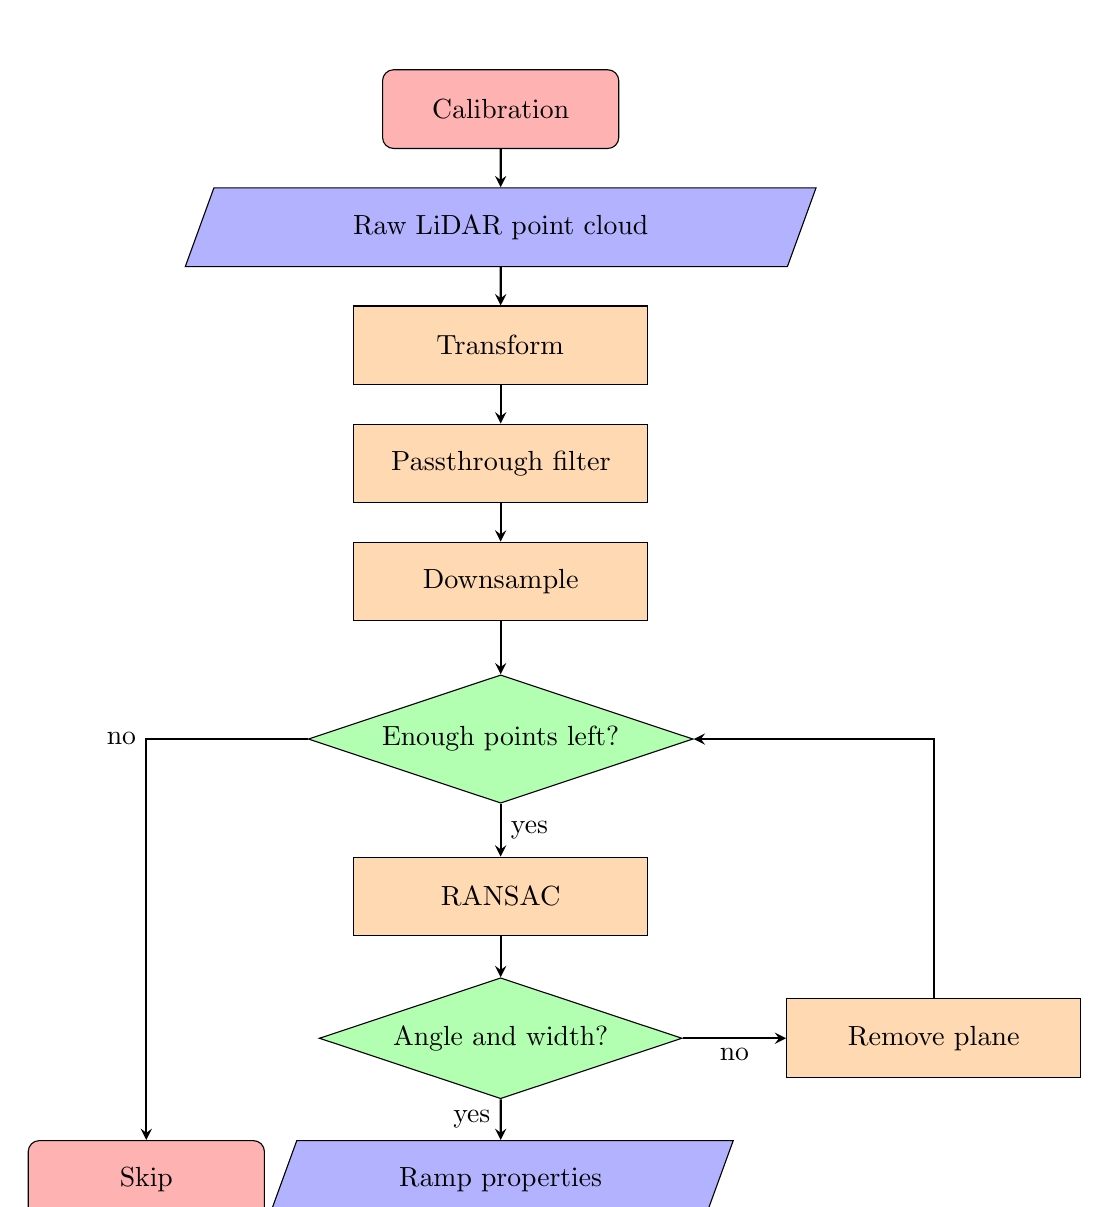
\begin{tikzpicture}[node distance=1.5cm]
    % \node (start) [startstop] {Start};
    % \node (raw) [io, below of=start] {Raw \acrshort{lidar} point cloud};
    \node (calibration) [startstop] {Calibration};
    \node (raw) [io, below of=calibration] {Raw LiDAR point cloud};
    \node (transform) [process, below of=raw] {Transform};
    \node (passthrough) [process, below of=transform] {Passthrough filter};
    \node (downsample) [process, below of=passthrough] {Downsample};
    \node (is_enough_points) [decision, below of=downsample, yshift=-0.5cm] {Enough points left?};
    \node (ransac) [process, below of=is_enough_points, yshift=-0.5cm] {RANSAC};
    \node (is_ramp) [decision, below of=ransac, yshift=-0.3cm] {Angle and width?};
    \node (reduce) [process, right of=is_ramp, xshift=4cm] {Remove plane};
    \node (rotmat) [io, below of=is_ramp, yshift=-0.3cm] {Ramp properties};
    \node (skip) [startstop, left of=rotmat, xshift=-3cm] {Skip};
    % \node (end) [startstop, below of=rotmat] {Stop};


    % Connect the nodes
    % \draw [arrow] (start) -- (raw);
    \draw [arrow] (calibration) -- (raw);
    \draw [arrow] (raw) -- (transform);
    \draw [arrow] (transform) -- (passthrough);
    \draw [arrow] (passthrough) -- (downsample);
    \draw [arrow] (downsample) -- (is_enough_points);
    \draw [arrow] (is_enough_points) -- node[anchor=west] {yes} (ransac);
    \draw [arrow] (is_enough_points) -| node[anchor=east] {no} (skip);
    \draw [arrow] (ransac) -- (is_ramp);
    \draw [arrow] (is_ramp) -- node[anchor=east] {yes} (rotmat);
    \draw [arrow] (is_ramp) -- node[anchor=north] {no} (reduce);
    \draw [arrow] (reduce) |- (is_enough_points);
    % \draw [arrow] (rotmat) -- (end);
\end{tikzpicture}
\end{document}
	\caption{Flow chart of the ramp detection algorithm using the \acrshort{lidar} sensor.}
	\label{fig:flowchart_lidar}
\end{figure}
Because the raw \gls{lidar} data is too big to allow for real time processing, preprocessing is necessary.
It consists of a passthrough filter to remove unwanted points (e.g. behind the car) and a voxel grid filter to downsample the point cloud.
Before the passthrough filter can be applied, the point cloud must be transformed to the car frame.
The in the previous section described calibration algorithm is performed once at the start and its returned rotation is then applied to every new measurement.\\
The passthrough filter then removes all the points which lie outside the specified x, y and z limits.
Because the car drives forward, only points in front of the car are of interest.
Furthermore, the points further away than a certain threshold are neglected, because the resolution and accuracy of the measurements of the \gls{lidar} decreases with increasing distance.
The ceiling points are removed by limiting the points in z-direction.
The exact values used for the passthrough filter can be seen along the other parameters in \cref{tab:lidar_params}.\\
The next step in reducing the point cloud size is the voxel grid filter \cite{Vosselman2004}.
The point cloud is converted into a 3D grid consisting of small cubes called voxels.
Each cube can contain multiple points or none, the size of the voxels (also known as leaf size) determines the resolution.
All the points inside a cube are then reduced to their most centroid point.
If the cube does not contain any points, it is neglected.
\subsubsection{Ramp detection}
Now that the point cloud size is reduced greatly the actual ramp detection can be performed with sufficient performance.
The \gls{ransac} algorithm usually detects the following types of planes: ceiling, ground, side wall or the desired ramp.
\gls{ransac} is applied iteratively until a plane of type ramp has been found.
If a plane of different type has been found, it gets removed and the \gls{ransac} algorithm is applied again.
To prevent an infinite loop, the algorithm will exit after either a certain number of iterations has been performed, or if after the removal of a plane not enough points are left in the point cloud.
For the implementation of the \gls{ransac} algorithm and the voxel grid filter the PCL library \cite{Rusu2011} has been used.\\
The accidental detection of the ceiling was already prevented during the passthrough filter step, where the ceiling points have been removed from the point cloud.
Wrong detections of the ground plane or side walls can be prevented by requiring the angle to be in a certain range.

\subsubsection{Ramp properties}
\iimprov{This section needs imporovement}
Beside the angle, the width of the plane (y-range) is being calculated and compared to the parameters, to make sure that the plane is a drivable ramp for cars and not e.g. a small ramp for wheelchairs \todo{no idea if wheel chair ramps are common in parking garages?}.
The distance to the ramp is estimated by taking the $n$ nearest points of the ramp plane and calculating their mean.
If a ramp has been detected, the estimated angle and distance from the car front to the beginning of the ramp are returned.\\
A visual representation of the algorithm is depicted in \cref{fig:flowchart_lidar}.
\iimprov{Explain flow chart better}
\isug{What happens with stairs?}
\itodo{Add down ramp detection}
\iimprov{Add some more algo parameters to table (full one in appendix)}
\begin{table}[H]
	\centering
	\caption{Used parameters for lidar algo}
	\label{tab:lidar_params}
	\begin{tabular}[t]{lc}
		\toprule
		\textbf{parameter} & \textbf{value}          \\
		\midrule
		\textbf{Passthrough filter}                  \\
		x                  & \SIrange{0}{30}{\metre} \\
		y                  & \SIrange{-2}{2}{\metre} \\
		z                  & \SIrange{-1}{2}{\metre} \\
		\midrule
		\textbf{Voxel filter}                        \\
		leaf size          & \SI{0.1}{\metre}        \\
		\midrule
		\textbf{\gls{ransac}}                        \\
		max iter           & 100                     \\
		distance threshold & \SI{0.11}{\metre}       \\
		normal distance w  & 0.01                    \\
		\midrule
		\textbf{rd}                                  \\
		angle              & \SIrange{3}{9}{\degree} \\
		width              & \SIrange{2}{6}{\metre}  \\
		$o$                & 4                       \\
		\bottomrule
	\end{tabular}
\end{table}%



\section{Camera only}
Detectron2 was used to identify the ramp in the images.
\todoin{\begin{itemize}
		\item Explain...
		\item Choice of detectron2
		\item Pretrained model
		\item Hyperparameters
		\item Data augmentation
		\item Labeling and stuff
	\end{itemize}}

\cite{Wu2019}
\dots limited data.
For the ... the detectron2 network is used.
\dots

Using transfer learning the training time of the model can be greatly reduced.
The COCO dataset is used for training.
\cite{Lin2014}

\chapter{Experimental Setup}
\label{ch:ExperimentalSetup}

\section{Sensors}
\subsection{\glsentrytext{imu}}
\missingfigure{Picture of myAHRS+ or/and ZED2i}
Two different \gls{imu}s will be used for the experiment.
The first one being the WITHROBOT myAHRS+, a low cost high performance \gls{ahrs}.
An \gls{ahrs} contains an \gls{imu} and outputs the raw data but also has an integrated Kalman filter which calculates the pose in form of quaternion or euler angles.
The second \gls{imu} used during the experiment is integrated in the ZED 2i Stereo camera.
The specifications of each \gls{imu} can be read in table
\begin{table}[ht]
	\centering
	\caption{Comparison of the two used \gls{imu}s}
	\label{tab:imu_datasheets}
	\begin{tabular}[t]{lcc}
		\toprule
		                            & \textbf{myAHRS+}                                       & \textbf{ZED 2i \gls{imu}}                              \\
		\midrule
		Accelerometer range         & $\pm\SI{16}{\g}$                                       & $\pm\SI{8}{\g}$                                        \\
		Gyroscope range             & $\pm\SI{2000}{\degree\per\second}$                     & $\pm\SI{1000}{\degree\per\second}$                     \\
		Magnetometer range          & $\pm\SI{1200}{\micro\tesla}$                           & $\pm\SI{2500}{\micro\tesla}$                           \\
		Rate                        & \SI{100}{\hertz}                                       & \SI{400}{\hertz}                                       \\
		Accelerometer noise density & \SI{4.502e-3}{\metre\per\second(1\per\sqrt{\second})}  & \SI{1.148e-3}{\metre\per\second(1\per\sqrt{\second})}  \\
		Accelerometer random walk   & \SI{7.337e-5}{\metre\per\second\squared\sqrt{\second}} & \SI{6.458e-5}{\metre\per\second\squared\sqrt{\second}} \\
		Gyroscope noise density     & \SI{1.674e-4}{\radian\per\sqrt{\second}}               & \SI{8.254e-5}{\radian\per\sqrt{\second}}               \\
		Gyroscope random walk       & \SI{5.042e-6}{\radian\per\second\sqrt{\second}}        & \SI{1.632e-7}{\radian\per\second\sqrt{\second}}        \\
		\bottomrule
	\end{tabular}
\end{table}%
\itodo{Add cite to manuals}
\iimprov{Values and units of random walk and noise density probably wrong (measured them myself)}
It offers an micro-USB interface and runs with up to \SI{100}{\Hz}.
It can capture a change of $\pm$2000 dps (degrees per second), $\pm$16 $g$ and $\pm$\SI{1200}{\micro\tesla}.
During the experiment only a fraction of this range is expected to be reached, hence the sensor seems suitable.
Besides the hardware the unit already has an Extended Kalman Filter (EKF) on board.
The EKF fuses the measurements of the three sensors and estimates a quaternion (and sth else?) from it.
But this will not be used.
\iimprov{More about both \gls{imu}}


\subsection{\glsentrytext{lidar}}
Two different \gls{lidar}s will be used during the experiment.
The RS-Bpearl and the Velodyne UltraPuck.
The most relevant specifications of the two \gls{lidar}s can be seen in table \ref{tab:lidar_datasheets}.
Both are mechanical \gls{lidar}s and have the same number of laser channels, but the Velodyne has a significant better vertical resolution, due to the smaller vertical \gls{fov}.
\begin{table}[ht]
	\centering
	% todo: Manual citation prop wrong
	\caption{Comparison of the two used \acrshort{lidar}s \cite{RoboSense2020}\cite{Velodyne2018}}
	\label{tab:lidar_datasheets}
	\begin{tabular}[t]{lcc}
		\toprule
		                      & \textbf{RS-Bpearl}          & \textbf{Velodyne Ultra Puck}                  \\
		\midrule
		Channels              & 32                          & 32                                            \\
		Range                 & \SI{100}{\metre}            & \SI{200}{\metre}                              \\
		Range accuracy        & $\pm\SI{3}{\centi\metre}$   & $\pm\SI{3}{\centi\metre}$                     \\
		Horizontal \gls{fov}  & \SI{360}{\degree}           & \SI{360}{\degree}                             \\
		Vertical \gls{fov}    & \SI{90}{\degree}            & \SI{40}{\degree} (\SIrange{-25}{15}{\degree}) \\
		Horizontal resolution & \SIrange{0.2}{0.4}{\degree} & \SIrange{0.1}{0.4}{\degree}                   \\
		Vertical resolution   & \SI{2.81}{\degree}          & \SI{0.33}{\degree}                            \\
		Frame rate            & \SIrange{10}{20}{\hertz}    & \SIrange{5}{20}{\hertz}                       \\
		Laser wavelength      & \SI{905}{\nano\metre}       & \SI{903}{\nano\metre}                         \\
		% \midrule
		Points per second     & 576,000                     & 600,000                                       \\
		\bottomrule
	\end{tabular}
\end{table}%
\begin{figure}[htb]
	\centering
	\begin{subfigure}{0.3\textwidth}
		\centering
		\includegraphics[width=\textwidth]{Robosense.png}
		\caption{Robosense RS-Bpearl \cite{RoboSense2020}}
		\label{fig:lidar_robosense}
	\end{subfigure}
	% \hfill
	\begin{subfigure}{0.3\textwidth}
		\centering
		\includegraphics[width=\textwidth]{Velodyne.png}
		\caption{Velodyne Ultra puck \cite{Velodyne2018}}
		\label{fig:lidar_velodyne}
	\end{subfigure}
	\caption{The two used \gls{lidar}s}
	\label{fig:lidars_used}
\end{figure}



\section{Sensor placement}
The \gls{imu} must be placed on a rigid point of the car, such that the \gls{imu}'s position stays always the same relative to the car.
Other then that it should also be placed in the transversal center? to guarantee that the centripetal acceleration is not skewed towards one side.
The \gls{imu} was placed on the roof center.
\begin{figure}[htpb]
	\centering
	\documentclass{standalone}
\usepackage{tikz}
\usepackage{tikz-dimline}		% Dimension (measure) lines for TikZ
\usetikzlibrary{angles, calc, decorations.pathmorphing, quotes, spy}

\begin{document}
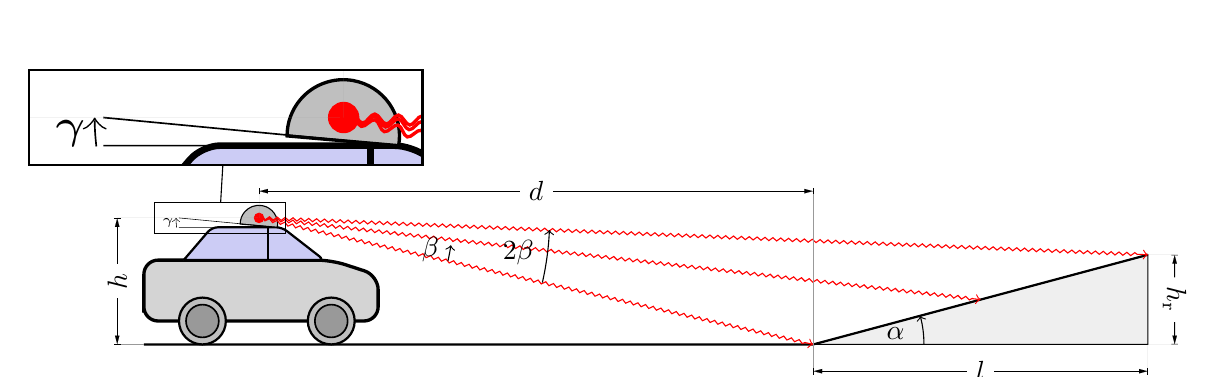
\begin{tikzpicture}[scale=0.85, spy using outlines={black, rectangle, magnification=3, width=5cm, height=1.2cm, connect spies}]
    % Define/Calc ramp parameters
    % Ramp length
    \def\rl{5};
    % Ramp angle [deg]
    \def\ra{15};
    % Ramp height
    \def\rh{{tan(\ra)*\rl}};
    % Distance of measurement line
    \def\dd{.4cm}

    % RAMP
    % Define the points
    \coordinate (A) at (0,0);
    \coordinate (B) at ($(A) + (\rl,0)$);
    \coordinate (C) at ($(B) + (0,\rh)$);
    % Draw and fill ramp
    \filldraw[draw=black, fill=lightgray!25] (A) -- (B) -- (C) -- cycle;
    % Draw angle
    \path (A) -- (B)
    pic[draw, ->, angle radius=40pt,
    angle eccentricity=0.75, "$\alpha$"]{angle=B--A--C};
    % Ground and helpers
    \coordinate (D) at ($(A) + (-10,0)$);
    \draw [thick] (D) -- (A) -- (C);

    % CAR
    \begin{scope}[scale=0.7]
        % Car height
        \def\ch{2}
        % Car length
        \def\cl{5}
        % Car body height
        \def\bh{\ch*0.65}
        % Roof length
        \def\rl{\cl*0.6}
        % Roof height
        \def\rh{\ch*0.35}
        % Car tilt angle
        \def\ct{6}
        % Anchor point is southwest
        \coordinate (b) at ($(D) + (0,0.5)$);
        % Offset to roof and wheels
        \coordinate (r) at ($(b) +(\cl*0.17,\ch*0.65)$);
        \coordinate (w) at ($(b) + (\cl*0.25,0)$);

        % Body
        \draw[black, fill=black!17, rounded corners=1.2ex, very thick]
        (b) -- ++(0,\bh) -- ++(\cl*1/5,0) --  ++(\cl*3/5,0) -- ++(\cl*1/5,-\bh*0.25)
        -- ++(0, -\bh*0.75) -- (b) -- cycle;
        % Roof
        \draw[very thick, rounded corners=0.5ex, fill=black!20!blue!20!white,thick]
        (r) -- ++(0.2*\rl,\rh) -- ++(0.5*\rl,0) -- ++(0.3*\rl,-\rh) -- (r);
        % \draw[thick] ($(r) + (\cl*0.5,\bh)$) -- ++(0,\rh);
        \draw[thick] (r)++(\rl*0.6,0) -- ++(0,\rh);

        % Wheels
        \draw[draw=black,fill=gray!50,thick] (w) circle (.5);
        \draw[draw=black,fill=gray!50,thick] (w) ++(\cl*0.55,0) circle (.5);
        % Inner wheels
        \draw[draw=black,fill=gray!80,semithick] (w) circle (.35);
        \draw[draw=black,fill=gray!80,semithick] (w) ++(\cl*0.55,0) circle (.35);

        % Lidar
        \draw[black, fill=gray!50] ($(r) + (\cl*0.40,\rh)$) coordinate (le) arc(-10:180:0.4) --cycle;

        % Car middle point
        \coordinate (m) at (\cl*0.5, \bh*0.5);
        % Lidar middle point
        \coordinate (lm) at ($(le) + (-0.39,0.2)$);
        \filldraw[red] (lm) circle(.1);
        % lidar mount angle
        % \draw (lm) -- ($(lm) + (-3, 0)$);
        % \path (A) -- (B)
        \coordinate (blob) at ($(le) + (-2.1, 0)$);
        \coordinate (blub) at ($(le) + (-2.1, 0.2)$);
        % \draw (blob) circle (.1);
        % \draw (blub) circle (.1);
        \draw[draw=black, very thin] (blob) -- (le) -- (blub)
        pic[draw, <-, angle radius=30pt,
        angle eccentricity=1.1, "\tiny $\gamma$"]{angle=blub--lm--blob};

        % Laser lines
        \draw[->,color=red,decorate,decoration={snake,amplitude=.2mm,segment length=1mm,post length=1mm}] (lm) -- (A);
        \draw[->,color=red,decorate,decoration={snake,amplitude=.2mm,segment length=1mm,post length=1mm}] (lm) -- ($(A)!0.5!(C)$);
        \draw[->,color=red,decorate,decoration={snake,amplitude=.2mm,segment length=1mm,post length=1mm}] (lm) -- ($(A)!1!(C)$);
        \path (lm) -- (A)
        pic[draw, ->, angle radius=70pt, angle eccentricity=0.9,
        "$\beta$"]{angle=A--lm--B};
        \path (lm) -- (C)
        pic[draw, ->, angle radius=105pt, angle eccentricity=0.9,
        "$2\beta$"]{angle=A--lm--C};
    \end{scope}

    % \dimline[extension start length=-\dd, extension end length=-\dd] {($(D)+(0,-\dd)$)}{($(A)+(0,-\dd)$)}{$d$};
    % \dimline[extension start length=\dd, extension end length=\dd] {($(A)+(0,-\dd)$)}{($(A)!0.4!(D)+(0,-\dd)$)}{$d$};
    \dimline[extension start length=\dd, extension end length=\dd+1.9cm] {($(lm)+(0,\dd)$)}{($(lm -| A)+(0,\dd)$)}{$d$};
    \dimline[extension start length=-\dd, extension end length=-\dd] {($(A)+(0,-\dd)$)}{($(B)+(0,-\dd)$)}{$l$};
    \dimline[extension start length=-\dd, extension end length=-\dd] {($(B)+(\dd,0)$)}{($(C)+(\dd,0)$)}{$h_\mathrm{r}$};
    \dimline[extension start length=\dd, extension end length=\dd+1.7cm] {($(D)+(-\dd,0)$)}{($(lm -| D)+(-\dd,0)$)}{$h$};
    % \draw (D) -- (lm -| D);
    % \dimline[extension start length=-\dd, extension end length=-\dd] {($(lm)+(\dd,0)$)}{($(C)+(\dd,0)$)}{$h_2$};
    % \dimline[extension start length=\dd, extension end length=\dd] {($(A)+(0,\dd)$)}{($(C)+(0,\dd)$)}{$d$};
    % \spy on ($(lm)!.05!(A)$) in node at (3,4);

    % \spy[black] on ($(lm) + (-0.42, 0)$) in node at (3,4);
    \spy on ($(lm) + (-0.5, 0)$) in node at ($(lm) + (-0.5, 1.5)$);

\end{tikzpicture}
\end{document}
	\caption{Mounting of the \acrshort{lidar}}
	\label{fig:tikz_lidar_mount}
\end{figure}
\begin{table}[htbp]
	\centering
	\caption{Some params}
	\label{tab:vals}
	\begin{tabular}[t]{clc}
		\toprule
		\textbf{Variable} & \textbf{Description}                                   & \textbf{Unit} \\
		\midrule
		$h_\mathrm{l} $   & \gls{lidar} height above ground                        & \si{\metre}   \\
		$d$               & Distance to ramp                                       & \si{\metre}   \\
		$h_\mathrm{r}$    & Height of ramp                                         & \si{\metre}   \\
		$l_\mathrm{w}$    & Light travel distance from ramp start to contact point & \si{\metre}   \\
		$d_\mathrm{w}$    & Distance from ramp start to contact point              & \si{\metre}   \\
		$\alpha$          & Ramp angle                                             & \si{\degree}  \\
		$\beta$           & \gls{lidar} mount angle                                & \si{\degree}  \\
		$\gamma$          & Tue angle?!                                            & \si{\degree}  \\
		$\epsilon$        & \gls{lidar} vertical resolution                        & \si{\degree}  \\
		$n$               & Number of laser channels                               &               \\
		\bottomrule
	\end{tabular}
\end{table}

The \gls{lidar} will be placed on top of the car, to get a greater \gls{fov}.
The pitch angle $\beta$ at which the \gls{lidar} will be mounted should be chosen such that the number of points in the area at the beginning of the ramp are maximized.
This allows for the most accurate distinction between planes of different inclination angles and therefore also a good distance estimation.
Because the distance to the ramp is not constant due to the movement of the car, the optimization can only be done for a specific distance.
The coordinates at which the lasers hit the ground and ramp depend on the height of the \gls{lidar} $h_\mathrm{l}$, the distance to the ramp $d$, the angle of the ramp $\alpha$, the angle $\beta$ at which the \gls{lidar} has been mounted on the car and finally on the vertical resolution and \gls{fov} of the \gls{lidar}.
The coordinates can be calculated in the following way.\\
The angle $\gamma$ between the NOT ground and each laser wave is defined as
\begin{equation}
	\gamma = \beta - i\epsilon
\end{equation}
with $i \in \mathbb{N}, 0\dots n$ being the "laserID" starting from the lowest opening angle and going to the highest.
On flat ground the distance at which the laser waves hit the ground can be calculated with
\begin{equation}
	x = \tan(\ang{90} - \gamma) h_\mathrm{l}.
	\label{eq:ground_points}
\end{equation}
With a ramp, the assumption from \ref{eq:ground_points} does not hold anymore.
The light does not travel as far.
The height above ground, when the light is at the beginning of the ramp can be calculated with
\begin{equation}
	h_\mathrm{w,start} = h_\mathrm{l} - d\tan(\gamma)
\end{equation}
The distance $l_\mathrm{w}$ which the light travels from the beginning of the ramp to the contact point with the ramp can be calculated using the law of sines
\begin{align}
	l_\mathrm{w} & = \frac{h_\mathrm{w,start} }{\sin(\alpha + \gamma)} \sin(\ang{90} - \alpha) \\
	             & = \frac{h_\mathrm{w,start} }{\sin(\alpha + \gamma)} \cos(-\alpha)
\end{align}
The travelled distance along the x-axis from the start of the ramp to the contact point is then
\begin{equation}
	d_\mathrm{w}  = l_\mathrm{w} \sin(\ang{90} - 2\alpha - \gamma)
\end{equation}
which results in the total x distance from the \gls{lidar}
\begin{equation}
	d_\mathrm{hit} = d + d_\mathrm{w}.
\end{equation}
\iquest{Instead of "long" derivation, just use the final equation?}
\begin{equation}
	d_\mathrm{hit} = d + \frac{h_\mathrm{l} - d\tan(\gamma)}{\sin(\alpha + \gamma)} \cos(-\alpha) \sin(\ang{90} - 2\alpha - \gamma)
\end{equation}
Using the formulas the optimal mounting pitch angle $\beta$ for the two \gls{lidar}s has been found with $\beta_\mathrm{velodyne} = \ang{0}$ and $\beta_\mathrm{robos} = \ang{20}$.
\iimprov{Improve text and table param description}


\section{Car}
The car used in the experiment is an eGolf 2017.
The car has been "hacked" which allows for the reading of the wheel ticks.
Because the ... mode is used, the output power of the motor is limited and the maximum speed is capped at \SI{5}{\kilo\metre\per\hour}.
The traversing of ramps is not possible and this mode, which is why a the normal mode was used for the recording where the ramp was fully driven up.
But in the normal driving mode the wheel speed readings were not available.
The car has a pc in the booth, at which the sensors were connected to.
\iimprov{Text is bad}
\missingfigure{Picture of eGolf}
\todoin{\begin{itemize}
		\item Some stats as height, track width etc, electric car hence less vibrations
		\item Connection setup (maybe own section or maybe not interesting at all)
	\end{itemize}
}



\section{Garage}
\missingfigure{Picture of ramps and/or figure of ramps showing angles}
\itodo{Think of a good way to measure the true angle of the ramps}
\chapter{Results}
\label{ch:Results}
% Do not write long version of imu or lidar acronym again
\glslocalunset{imu}
\glslocalunset{lidar}
\itodo{Chapter description}

\section{Evaluation concept}
During each test drive the measurements of the accelerometer and gyroscope of the \gls{imu} (of both \glspl{imu}, myAHRS+ and of the \gls{imu} integrated in the ZED 2i camera), the camera image of the ZED 2i camera and the point cloud generated by the \gls{lidar} are recorded.
Only one \gls{lidar} could be mounted at a time, so the Velodyne UltraPuck was used for most test drives, but two recordings were also made using the Robosense.
Furthermore, the wheel speeds were recorded when available, which was only the case when driving a ramp down or only half-way up, as mentioned in \cref{sec:car}.\\
To prevent an overfitting of the model it is important to have different test scenarios.
As mentioned in \cref{sec:garage}, four different ramps were available to test the model.
For the evaluation of the \gls{imu} only the ramps A B, and D will be used.
Multiple test drives were made for each scenario, the most drives where performed on ramp A.
Because the wheel speed sensor measurements are needed for some methods, which are only available in a special mode where the power of the car is very limited, the ramps A and B could only be driven halfway up.
But a full recording including the wheel speed measurements could be done for ramp D and A, when driving down.\\
The algorithms using the \gls{lidar} and camera only detect ramps going up, so only the ramps A, B and C were used.
Furthermore, a test drive without any ramps in sight was made to test if false positives are being detected.



\section{Reference data}
To evaluate the performance of the different algorithms a reference is necessary.
The open-source \gls{ros} package \texttt{hdl\_graph\_slam}~\footnote{\url{https://github.com/koide3/hdl_graph_slam}} is used for this task.
It is based on 3D graph \gls{slam} and uses the \gls{lidar} data to map the environment and estimate the pose (position and orientation) of the car.
It uses NDT scan matching-based odometry estimation with loop detection.
The point cloud of common features at time $t$ is compared to the point cloud from the time $t-1$ and matched against each other.
The algorithm then estimates the translation and orientation difference between those two point clouds.
In ref.~\cite{Akpnar2021} the accuracy of the HDL Graph \gls{slam} was tested and a mean error of \SI{4}{\cm} and a standard deviation of \SI{5}{\cm} was measured for an indoor scenario.\\
From the pose information of the HDL Graph \gls{slam} the pitch angle of the car can be calculated and be used as a reference for the road grade, to evaluate the performance of the different \gls{imu}-based methods.
Because the \gls{lidar} only records at \SI{10}{\hertz} and thus the estimation of the HDL Graph \gls{slam} also only updates at \SI{10}{\hertz}, but the other sensors record from \SIrange{100}{400}{\hertz}, the estimate was upsampled using a Fourier method.
Beside estimating the road grade, the \gls{imu} is used to estimate the angle and length of the ramp.
Both of those values can be extracted from the generated point cloud map, by measuring the distance between the corresponding points.
Because the ramp angle is not constant, the average angle of the ramp is used as reference.
The average angle $\alpha$ is calculated by measuring the length and height of the ramp and using the law of sines
\begin{equation}
	\gls{ramp_ang} = \arcsin\left(\frac{h_\mathrm{ramp}}{l_\mathrm{ramp}}\right).
\end{equation}
The \gls{lidar} is used to detect and track the distance to the ramp and also to estimate the angle, width and length.
For the evaluation of the tracking accuracy, the generated map and pose provided by the HDL Graph \gls{slam} is used again.
In the generated point cloud map, the ramp region was marked manually by visual inspection.
Then, using the position of the car, provided by the \gls{slam}, the true distance to the beginning of the ramp could be calculated, by measuring the distance of the current position to the beginning of the ramp for each frame.\\
An example of the point cloud map generated by the \texttt{hdl\_graph\_slam} package is shown in \cref{fig:pcd_rviz}.
The color of the points gives information about the z-value (height information) of the points.
The ramp region is marked by the greater and brighter points and the white arrows visualize the trajectory of the car.
In this example the car was driven only half-way up the ramp.
\begin{figure}[htbp]
	\centering
	\includegraphics[width=.95\linewidth]{pcd_rviz.png}
	\caption[Generated point cloud]{The by the \texttt{hdl\_graph\_slam} package generated point cloud map. The white arrows visualize the trajectory of the car.}
	\label{fig:pcd_rviz}
\end{figure}



\section{Performance measures}
Using the \gls{imu}, the pitch angle of the car is estimated over time.
The goodness of the fit between the estimation $\hat{y} = (\hat{y}_i, \dots, \hat{y}_n)^\intercal$ and the reference $y = (y_i, \dots, y_n)^\intercal$ can then be described by the \gls{rmse}
\begin{equation}
	RMSE = \sqrt{\frac{1}{n}\sum_{i = 1}^n(\hat{y}_i - y_i)^2},
\end{equation}
which quantifies how much the predicted values differ from the reference value on average.
It is defined in the range $[0, \infty)$, with a value of 0 indicating a perfect fit.
The same can be applied to the estimation for the angle, width, length and distance to the ramp by the \gls{lidar}-based method.
The only difference is that the reference angle, width and length are constant and thus the \gls{rmse} is basically the same as the standard deviation in this case.\\
Furthermore, the coefficient of determination $R^2$ is used to evaluate the pitch angle estimation
\begin{equation}
	R^2 = 1 - \frac{\sum\limits_{i = 1}^n(\hat{y}_i - y_i)^2}{\sum\limits_{i = 1}^n(\hat{y}_i - \overline{y})^2},
\end{equation}
where $\overline{y}$ indicates the mean of the reference.
The goodness of the fit is described in the range from 0 to 1, where 1 describes a perfect fit.
\iquest{True positives, sensitvity and stuff here or later?}



\section{\glsentryshort{imu}}
\itodo{Brief overview}

\subsection{Road grade estimation}
The ramp detection using the \gls{imu} relies on the correct estimation of the road grade angle.
Hence, the evaluation of the goodness of the estimation is necessary to determine the performance of the ramp detection algorithm.\\
Different recordings of different ramps were made, but the results will be discussed on only two test drives.
Furthermore, two different \glspl{imu} were used, but only the measurements of one \gls{imu} will be used to present the results, since both produced similar results.
Because the \gls{imu} of the ZED camera is slightly more accurate as shown in \cref{tab:imu_datasheets} only those measurements will be used.
In the first drive the car was accelerated from stand still and drove up ramp A about half-way up.
As explained in \cref{sec:car}, the ramp could not be driven completely, due to the need of the odometer readings, which are only available when the motor output is limited.
The result of using only the raw measurements of the \gls{imu} for the pitch angle calculation is shown in \cref{fig:imu_raw_angle}.
\begin{figure}[htb]
	\centering
	\includegraphics[width=.9\linewidth]{imu_raw_angle.pdf}
	\caption[Angle estimation using raw measurements]{Pitch angle estimation from the raw accelerometer and gyroscope measurements. The drive did start from stand still and did end in the middle of the ramp.}
	\label{fig:imu_raw_angle}
\end{figure}
The measurement by the accelerometer is very noisy and is easily influenced by accelerations other than gravity, which can be seen at time \SIrange{2}{4}{\second}, where the car started driving.
The gyroscope on the other hand provides good short-term accuracy and is not influenced by other accelerations, but is slowly drifting over time.
The reference is taken from the orientation estimation of the \texttt{hdl\_graph\_slam} package, which uses the \gls{lidar} data.
The time frame during which the car was on the ramp is marked by the yellow coloring.
The beginning of the ramp is classified as the point, where the reference data surpasses \ang{1.5}.\\
The gravity method tries to overcome the problem of the accelerometer of also detecting other accelerations than gravity, by subtracting the car's acceleration from the accelerometer measurement.
The car's acceleration $\vb{a}_\mathrm{odom,x} $ was calculated by calculating the derivate of the low-pass filtered car velocity $v_\mathrm{car} $, which was calculated from the wheel speed measurements.
Figure \ref{fig:imu_odometer_acc} shows the (low-pass filtered) acceleration measured by the \gls{imu} along the x-axis and the (low-pass filtered) car's acceleration.
\begin{figure}[htb]
	\centering
	\includegraphics[width=.9\linewidth]{imu_odometer_acc.pdf}
	\caption[Acceleration from \gls{imu} and odometer]{The measured acceleration in x-direction by the \gls{imu} and the acceleration derived from the wheel speed measurements and the difference between both.}
	\label{fig:imu_odometer_acc}
\end{figure}
$\vb{a}_\mathrm{grav,x} $ is the acceleration measured by the \gls{imu} from which the car acceleration $\vb{a}_\mathrm{odom,x} $ was subtracted.
It can be seen, that especially at the beginning of the ramp (\SIrange{21}{23}{\second}) the gravity method shows it advantages.
The deceleration before entering the ramp is measured by both sensors and thus cancels out each other.
The same can be seen in the initial acceleration phase, where the car starts to drive from still stand (\SIrange[]{2}{4}{\second}).
Although both sensor are synchronized in time, the \gls{imu} senses the acceleration earlier than the wheel speed sensors which leads to a slight pike.
This could be due to the wheel speed sensors having a certain velocity threshold, below which they do not pick up any changes.
Other reasons for the difference could be, that other forces than the one from the car are present, e.g. from the suspension of the car or vibrations due to the road quality, which are not measured by the wheel speed sensors.
Also, the approximations made by calculating the finite difference of the car velocity to get the car acceleration have a negative influence on the result.
The resulting angle from the acceleration can be seen in \cref{fig:imu_odometer_angle}.
\begin{figure}[htbp]
	\centering
	\includegraphics[width=.9\linewidth]{imu_odometer_angle.pdf}
	\caption[Angle estimation using the gravity method]{Pitch angle estimation using only the accelerometer compared to the gravity method, which additionally uses the wheel speed measurements.}
	\label{fig:imu_odometer_angle}
\end{figure}
It can be seen that the gravity method improves the estimation accuracy significantly, compared to when only using the accelerometer data.
Especially the angle at the start and on the ramp is more accurately described when adding the odometer data to the accelerometer data for the calculation.
But it can also be seen that the time synchronization between both signals is important, as seen in during the initial acceleration phase.
Here, the subtraction leads to a negative value, which neither sensor had measured.\\
Another way to improve the estimation is using a complementary filter.
The results of which are shown in \cref{fig:imu_raw_compl_angle}.
Those are the results of a new drive, where the car was driven the ramp D and afterwards ramp A down.
\begin{figure}[htb]
	\centering
	\begin{subfigure}{1\textwidth}
		\centering
		\includegraphics[width=0.9\linewidth]{imu_raw_compl_angle.pdf}
		\caption{Pitch angle estimation using the complementary filter compared to using the raw measurements.}
		\label{fig:imu_raw_compl_angle}
	\end{subfigure}
	
	% \bigskip
	\begin{subfigure}{1\textwidth}
		\centering
		\includegraphics[width=0.9\linewidth]{imu_grav_compl_angle.pdf}
		\caption{Pitch angle estimation comparison of the other methods.}
		\label{fig:imu_grav_compl_angle}
	\end{subfigure}
	\caption{Comparison of different methods to estimate the pitch angle. Two different ramps were driven down successively.}
\end{figure}
\itodo{Probably remove compl grav filter from plot and do not mention it anywhere}
The complementary filter uses the estimation of the gyroscope measurements and corrects them using the accelerometer measurements to prevent drift.
It can be seen that the estimation using the complementary filter closely follows the reference except for the part between the two ramps (\SIrange{30}{60}{\second}).
Also, it has no offset at the end, unlike the estimation from the gyroscope data.\\
Other methods applied to the recordings of the same ride are shown in \cref{fig:imu_grav_compl_angle}.
The gravity method reduces the spikes of the raw accelerometer estimation, but introduces some new errors due to the odometer readings being slightly shifted in time in regard to the accelerometer readings.
\itodo{Check text below}
The gravity complementary filter which fuses the estimation from the gravity method instead of only the accelerometer data together with the gyroscope data achieves the best results.
The filer gain could be reduced such that the estimation of the gravity method can be trusted more because it peaks less.
This makes the estimation more responsive to changes.\\
The metrics to evaluate the different methods, when driving up a ramp, is shown in \cref{tab:eval_table_imu_up}.
\itodo{Describe results shown in table}
\iimprov{Maybe mark best result for each column}
\itodo{Create new tables with avg angle estimation and length estimation (going down)}
\begin{table}[htb]
	\centering
	\caption{Performance measures up ZED \gls{imu}}
	\label{tab:eval_table_imu_up}
	\resizebox{\textwidth}{!}{
		\begin{tabular}[t]{lcccccccc}
			\toprule
			\textbf{Properties} & \multicolumn{4}{c}{\textbf{Ramp A}} & \multicolumn{4}{c}{\textbf{Ramp B}}                                                                                                                           \\
			\midrule
			Angle               & \multicolumn{4}{c}{?}               & \multicolumn{4}{c}{?}                                                                                                                                         \\
			\hline
			\textbf{Method}     & \textbf{RMSE}                       & $\mathbf{R^2}$                      & $\mathbf{error_{max}}$ & \textbf{Angle} & \textbf{RMSE}    & $\mathbf{R^2}$   & $\mathbf{error_{max}}$ & \textbf{Angle} \\
			\cmidrule(lr){2-5}   \cmidrule(lr){6-9}
			Accelerometer       & 0.875                               & 0.675                               & 4.944                  & 7.74           & 0.650            & 0.787            & 3.378                  & 6.93           \\
			Gyroscope           & 0.508                               & 0.905                               & 1.373                  & 4.78           & 0.768            & 0.802            & $\mathbf{1.594  }$     & 4.34           \\
			Acceleration method & 0.357                               & 0.954                               & 2.482                  & 7.95           & 0.351            & $\mathbf{0.955}$ & 1.707                  & 7.06           \\
			Complementary       & $\mathbf{0.273} $                   & $\mathbf{0.976}$                    & $\mathbf{1.231 }$      & 4.96           & $\mathbf{0.324}$ & 0.952            & 1.647                  & 4.92           \\
			% Complementary grav  & 0.371                               & 0.948                               & 1.990                  & 6.54           & 0.358            & 0.951            & 1.211                  & 6.55           \\
			\bottomrule
		\end{tabular}
	}
\end{table}
\begin{table}[htb]
	\centering
	\caption{Performance measures down ZED \gls{imu}}
	\label{tab:eval_table_imu_down}
	\resizebox{\textwidth}{!}{
		\begin{tabular}[t]{lcccccccc}
			\toprule
			\textbf{Properties} & \multicolumn{4}{c}{\textbf{Ramp C}} & \multicolumn{4}{c}{\textbf{Ramp A}}                                                                                                                      \\
			\midrule
			Angle               & \multicolumn{4}{c}{?}               & \multicolumn{4}{c}{?}                                                                                                                                    \\
			\hline
			\textbf{Method}     & \textbf{RMSE}                       & $\mathbf{R^2}$                      & $\mathbf{error_{max}}$ & \textbf{Angle} & \textbf{RMSE} & $\mathbf{R^2}$ & $\mathbf{error_{max}}$ & \textbf{Angle} \\
			\cmidrule(lr){2-5}   \cmidrule(lr){6-9}
			Accelerometer       & 0.894                               & 0.746                               & 8.291                  & 7.74           & 0.938         & 0.784          & 3.967                  & 6.93           \\
			Gyroscope           & 0.219                               & 0.990                               & 0.736                  & 4.78           & 0.784         & 0.867          & 1.481                  & 4.34           \\
			Acceleration method & 0.369                               & 0.964                               & 2.211                  & 7.95           & 0.719         & 0.872          & 2.136                  & 7.06           \\
			Complementary       & 0.327                               & 0.977                               & 1.184                  & 4.96           & 0.753         & 0.862          & 2.131                  & 4.92           \\
			% Complementary grav& 0.328 & 0.977 & 1.190     & 6.54        & 0.754 & 0.862 & 2.142      & 6.55           \\
			\bottomrule
		\end{tabular}
	}
\end{table}


\subsection{Ramp properties estimation}
\iquest{Ramp angle estimation already discussed in table or not?}
As discussed in \cref{ssec:ramp_detection_imu}, the length of the ramp can be estimated by integrating the velocity of the car over the time interval between the start and end of the ramp.
The velocity can be estimated in two different ways.
Either by using the wheel speed measurements, or by integrating the accelerometer measurements.
For the evaluation of the accuracy of the estimation, recordings of a drive with a full traverse of a ramp is necessary.
As mentioned in ?, this is only possible when driving down.
Ramp D is used for this evaluation, the first part of the drive show in \cref{fig:imu_raw_compl_angle}.
In \cref{fig:imu_distance_velocity} different methods to estimate the velocity of the car are shown.
\begin{figure}[htb]
	\centering
	\begin{subfigure}{1\textwidth}
		\centering
		\includegraphics[width=0.9\linewidth]{imu_distance_velocity.pdf}
		\caption{Estimated car velocity calculated from the wheel speed measurements and the accelerometer data.}
		\label{fig:imu_distance_velocity}
	\end{subfigure}
	
	% \bigskip
	\begin{subfigure}{1\textwidth}
		\centering
		\includegraphics[width=0.9\linewidth]{imu_distance_position.pdf}
		\caption{The integration of the velocity leads to the travelled distance.}
		\label{fig:imu_distance_position}
	\end{subfigure}
	\caption{Comparison of different methods to estimate the length of the ramp.}
\end{figure}
$v_\mathrm{car}$ is the velocity calculated from the wheel speed measurements using \cref{eq:v_car}.
The other three methods are based on the integration of the accelerometer measurements.
$v_\mathrm{car}$ is the result of integrating the raw accelerometer measurements $\vb{a}_x$.
Because the raw signal also contains the gravity component, the estimation is not correct anymore when entering the ramp.
Up until the point where the car enters the ramp both estimation are very similar, but during the phase on the ramp the acceleration disturbs the estimation.
This problem is partially solved by $v_\mathrm{car, grav}$, which eliminates the gravity component by subtracting it using the pitch angle of the car, according to \cref{eq:acc_from_imu_wo_grav}.
The angle estimation using the complementary filter method is used in \cref{eq:acc_from_imu_wo_grav}.
Because the estimation of the angle is not correct at the start of the acceleration (\SIrange{3}{5}{\second}), an error is introduced.
As it can be seen in \cref{fig:imu_raw_compl_angle} the angle is slightly overestimated by the complementary filter during the acceleration phase.
This leads according to \cref{eq:acc_from_imu_wo_grav} to an underestimation of the acceleration, and thus also an underestimation of the velocity.
Due to the integration the error is cumulated over time and increases with the time.
This error can be fixed by introducing a new method, which ignores the initial acceleration phase, the results of which are visualized by $v_\mathrm{acc, grav, later}$.
The estimation of the distance for the different methods is shown in \cref{fig:imu_distance_position}.
Since the distance is calculated from the velocity, an error is cumulated over time.
This can be seen in both $d_\mathrm{acc}$ and $d_\mathrm{acc, grav}$.\\
The actual length of the ramp is calculated by subtracting the position of the car at the end of the ramp from the position at the start of the ramp.
The results for the different methods are shown in \cref{tab:ramp_length}.

\begin{table}[htb]
	\centering
	\caption[Ramp length]{The estimation of the ramp length using different methods.}
	\label{tab:ramp_length}
	\begin{tabular}[t]{ccc}
		\toprule
		\textbf{Method}                & \textbf{Length}    & \textbf{error} \\
		\midrule
		$d_\mathrm{car} $              & \SI{12.88}{\metre} & 0              \\
		$d_\mathrm{acc} $              & \SI{-8.44}{\metre} & 0              \\
		$d_\mathrm{acc, grav, } $      & \SI{4.52}{\metre}  & 0              \\
		$d_\mathrm{acc, grav, later} $ & \SI{12.85}{\metre} & 0              \\
		\bottomrule
	\end{tabular}
\end{table}



\todoin{\begin{itemize}
		\item Tune parameters
		\item Add distance measurement (for full drives)
		\item Ramp A = uc2s, Ramp B = us2c, Ramp C = dd2r, Ramp D = ds2c
	\end{itemize}}

\newpage
\section{Ramp detection (\glsentryshort{lidar})}
The \gls{lidar} is used to detect if a ramp is visible, track the position to the ramp as well as to estimate the angle and width of the ramp.
Due to the setup it was only possible to mount one \gls{lidar} at a time.
To get the best possible results the \gls{lidar} with the best resolution, especially in vertical direction, should be used.
A comparison of the resolution of the two \glspl{lidar} can be seen in \cref{fig:lidar_resolution_eval}.
\begin{figure}[htbp]
	\centering
	\begin{subfigure}{1\textwidth}
		\centering
		\includegraphics[width=.9\linewidth]{lidar_resolution_velodyne_eval.pdf}
		\caption{Velodyne}
		\label{fig:lidar_resolution_velodyne_eval}
	\end{subfigure}
	
	\begin{subfigure}{1\textwidth}
		\centering
		\includegraphics[width=.9\linewidth]{lidar_resolution_robos_eval.pdf}
		\caption{Robosense}
		\label{fig:lidar_resolution_robos_eval}
	\end{subfigure}
	\caption{Resolution comparison of the two \glspl{lidar}. The ramp region is framed in black. The Velodyne \gls{lidar} has a higher resolution.}
	\label{fig:lidar_resolution_eval}
\end{figure}
Here, a top-down view on the ramp of the points measured by the \gls{lidar} at a distance of \SI{7}{\metre} to the ramp is shown.
The blue points visualize all the points which were visible to the ramp detection algorithm after the downsampling and pass through filter has been applied.
The points marked red symbolize the points that were then detected as part of the ramp by the algorithm.
The ramp region is framed in black and was drawn manually by visually inspecting the by the \texttt{hdl\_graph\_slam} package generated point cloud.
The Velodyne \gls{lidar}, shown in \cref{fig:lidar_resolution_velodyne_eval}, provides many more lines compared to the Robosense, shown in \cref{fig:lidar_resolution_robos_eval}.
Hence, only the results produced using the Velodyne \gls{lidar} will be discussed from here on.\\
\itodo{Also explain sensitivity and stuff and prob replace tp and fp in table with it}
The detection rate is evaluated by using the number of \glspl{tp} and \glspl{fp}.
A frame is labeled as \gls{tp} if the ramp is visible to the \gls{lidar}, the algorithm detected a ramp and at least 50\% of the detected points actually lie inside the ramp region.
Analogously, a frame is classified as \gls{fp}, when a ramp was detected even though it was not visible or if less than 50\% of the detected points lie inside the ramp region.\\
The true distance to the ramp is measured by calculating the distance from the car's current position, which is provided by the \texttt{hdl\_graph\_slam} package, to the beginning of the ramp.
This value is used to evaluate performance of the tracking algorithm, by calculating the \gls{rmse} between this ground truth value and the estimated value.
The \gls{rmse} is also used to evaluate the accuracy of the angle, width and length estimation.
The estimated values are compared to values measured in the point cloud.\\
Since the resolution improves the closer the car gets to the ramp, the evaluation is divided into distance intervals of \SI{5}{\metre} of length.
The results for three different drives are shown in \cref{tab:eval_table_lidar}.
Each drive started about \SI{30}{\metre} from the ramp.
It can be seen that the detection works very well if the distance to the ramp is \SI{20}{\metre} or less.
For the ramp C? it can be seen, that the detection is only reliable when the car is less than \SI{15}{\metre} away from the ramp.
This can be explained by the taken path during the recording, which was started at an offset in y-direction to the ramp.
Due to the passthrough filter the ramp was thus not visible for the algorithm.\\
\todoin{\begin{itemize}
		\item Run script again, with correct true values (ramp angle and width)
		\item Right now same width and angle assumed for all ramps (and val is also wrong)
	\end{itemize}}
\iquest{Should TP and FP be replaced by precision and recall?}
\begin{table}[htbp]
	\centering
	\caption{Performance evaluation}
	\label{tab:eval_table_lidar}
	\begin{tabular}[t]{cccccccc}
		\toprule
		\textbf{Ramp}          & \textbf{Distance}        & \textbf{Frames} & \textbf{TP \%} & \textbf{FP \%} & $\textbf{RMSE}_d$  & $\textbf{RMSE}_w$ & $\textbf{RMSE}_\theta$ \\
		\midrule
		\multirow{6}{*}{u c2s} & \SIrange{0}{5}{\metre}   & 116             & 100.00\%       & 0.00\%         & \SI{0.73}{\metre}  & \SI{0.03}{\metre} & \SI{0.31}{\degree}     \\
		                       & \SIrange{5}{10}{\metre}  & 117             & 100.00\%       & 0.00\%         & \SI{0.73}{\metre}  & \SI{0.04}{\metre} & \SI{0.30}{\degree}     \\
		                       & \SIrange{10}{15}{\metre} & 116             & 100.00\%       & 0.00\%         & \SI{0.77}{\metre}  & \SI{0.07}{\metre} & \SI{0.34}{\degree}     \\
		                       & \SIrange{15}{20}{\metre} & 123             & 100.00\%       & 0.00\%         & \SI{1.07}{\metre}  & \SI{0.05}{\metre} & \SI{0.27}{\degree}     \\
		                       & \SIrange{20}{25}{\metre} & 140             & 99.23\%        & 0.00\%         & \SI{2.06}{\metre}  & \SI{0.12}{\metre} & \SI{0.65}{\degree}     \\
		                       & \SIrange{25}{30}{\metre} & 50              & 59.78\%        & 0.00\%         & \SI{1.66}{\metre}  & \SI{0.25}{\metre} & \SI{1.79}{\degree}     \\
		\hline
		\multirow{6}{*}{u s2c} & \SIrange{0}{5}{\metre}   & 62              & 100.00\%       & 0.00\%         & \SI{0.75}{\metre}  & \SI{0.02}{\metre} & \SI{0.52}{\degree}     \\
		                       & \SIrange{5}{10}{\metre}  & 62              & 100.00\%       & 0.00\%         & \SI{0.84}{\metre}  & \SI{0.02}{\metre} & \SI{0.53}{\degree}     \\
		                       & \SIrange{10}{15}{\metre} & 59              & 100.00\%       & 0.00\%         & \SI{0.89}{\metre}  & \SI{0.02}{\metre} & \SI{0.51}{\degree}     \\
		                       & \SIrange{15}{20}{\metre} & 61              & 97.92\%        & 2.08\%         & \SI{2.75}{\metre}  & \SI{0.02}{\metre} & \SI{0.68}{\degree}     \\
		                       & \SIrange{20}{25}{\metre} & 61              & 97.83\%        & 2.17\%         & \SI{3.69}{\metre}  & \SI{0.12}{\metre} & \SI{0.90}{\degree}     \\
		                       & \SIrange{25}{30}{\metre} & 59              & 42.75\%        & 0.00\%         & \SI{2.36}{\metre}  & \SI{0.90}{\metre} & \SI{1.82}{\degree}     \\
		\hline
		\multirow{6}{*}{u d2e} & \SIrange{0}{5}{\metre}   & 21              & 100.00\%       & 0.00\%         & \SI{0.94}{\metre}  & \SI{0.05}{\metre} & \SI{0.64}{\degree}     \\
		                       & \SIrange{5}{10}{\metre}  & 23              & 100.00\%       & 0.00\%         & \SI{0.79}{\metre}  & \SI{0.11}{\metre} & \SI{0.50}{\degree}     \\
		                       & \SIrange{10}{15}{\metre} & 28              & 100.00\%       & 0.00\%         & \SI{0.75}{\metre}  & \SI{0.10}{\metre} & \SI{0.44}{\degree}     \\
		                       & \SIrange{15}{20}{\metre} & 27              & 37.04\%        & 3.70\%         & \SI{2.59}{\metre}  & \SI{0.18}{\metre} & \SI{1.11}{\degree}     \\
		                       & \SIrange{20}{25}{\metre} & 29              & 0.00\%         & 3.45\%         & \SI{19.83}{\metre} & \SI{0.04}{\metre} & \SI{3.28}{\degree}     \\
		                       & \SIrange{25}{30}{\metre} & 28              & 10.71\%        & 0.00\%         & \SI{1.87}{\metre}  & \SI{0.25}{\metre} & \SI{1.91}{\degree}     \\
		\bottomrule
	\end{tabular}
\end{table}
The estimated ramp properties and distance to the ramp for one exemplary ride are shown in \cref{fig:lidar_eval}.
In \cref{fig:lidar_distance_eval} the estimated distance is shown in comparison to the reference distance provided by the \texttt{hdl\_graph\_slam} package.
The error reduces when the car is closer to the ramp.
Interestingly the value of the estimated distance seems to hold itself for several \si{\metre}.
This is most probably due to the vertical resolution of the \gls{lidar}.
Because the vertical resolution is not linear, the most lines are centered around the middle of the opening angle of the \gls{lidar}, which is -\ang{5} for the Velodyne.
Hence, only few lines fall into the region at the start of the ramp.
The distance to the ramp is calculated by measuring the distance from the car to the $n$ closest points which have been identified as part of the ramp.
Therefore, the distance can only be updated if a line which has previously hit the ground now hits the ramp.\\
Fig. \ref{fig:lidar_angle_eval} shows the difference between the estimated angle and the HOW measured angle.
It can be seen that the estimation varies by about \ang{1} if the distance is less than \SI{20}{\metre}.
The angle is almost exclusively underestimated (OR OVER?), which could be due to the fact that the measurement was wrong.\\
The estimated width at different distances to the ramp can be seen in \cref{fig:lidar_width_eval}.
The error is very small compared to the tracking error and lies in the order of \SI{10}{\cm}.
This is because the horizontal resolution is significantly better than the vertical resolution.
Note that the estimated width is the width of the whole ramp and not only the width of the drivable part.\\
\begin{figure}[htbp]
	\centering
	\begin{subfigure}{1\textwidth}
		\centering
		\includegraphics[width=.9\linewidth]{lidar_distance_eval.pdf}
		\caption{Distance to the ramp}
		\label{fig:lidar_distance_eval}
	\end{subfigure}
	
	\begin{subfigure}{1\textwidth}
		\centering
		\includegraphics[width=.9\linewidth]{lidar_angle_eval.pdf}
		\caption{Angle of the ramp}
		\label{fig:lidar_angle_eval}
	\end{subfigure}
	
	\begin{subfigure}{1\textwidth}
		\centering
		\includegraphics[width=.9\linewidth]{lidar_width_eval.pdf}
		\caption{Width of the ramp}
		\label{fig:lidar_width_eval}
	\end{subfigure}
	\caption{Estimated ramp properties and tracking of the ramp over ? using Velodyne}
	\label{fig:lidar_eval}
\end{figure}
An visualization of the detection algorithm can be seen in \cref{fig:points_projection}.
Here, the point cloud generated by the \gls{lidar} is projected onto to the camera image.
The quality of the projection depends on the accuracy of the measured translation and orientation difference between both sensors.
It can be seen that it is not perfect, e.g. the points do not quite match the camera image at the left pillar or the pipe on the ceiling.
Nonetheless it gives a good indication of what the \gls{lidar} actually sees.
The coloring of the point indicates the distance from the \gls{lidar} to the points.
Objects far away are marked by yellow points and nearby objects by blue points.
The green points were identified as part of the ramp by the algorithm.
It mostly fits the actual ramp very well.
The previously mentioned problem of the vertical resolution is clearly visible here.
While the density of the laser lines is sufficient in the ramp region, the start of the ramp and especially the ground is covered by very few lines.
This makes the precise tracking of the distance to the ramp difficult.
\begin{figure}[htbp]
	\centering
	\includegraphics[width=1\linewidth]{points_projection.pdf}
	\caption{Lidar points projected into the camera image. The green points were identified as part of a ramp.}
	\label{fig:points_projection}
\end{figure}



\section{Camera}
The camera was used to detect the ramp and mask the region.
\begin{figure}[htbp]
	\centering
	\includegraphics[width=1\linewidth]{camera_detection_compare}
	\caption{Machine learning}
	\label{fig:camera_detection_compare}
\end{figure}
\begin{figure}[htbp]
	\centering
	\includegraphics[clip, trim=5cm 1cm 5cm 6cm, width=1\linewidth]{points_prokection_mask.pdf}
	\caption{Machine learning}
	\label{fig:points_prokection_mask}
\end{figure}
\begin{equation}
	\text{Precision} = \frac{TP}{TP+FP}
\end{equation}
\begin{equation}
	\text{Recall} = \frac{TP}{TP+FN}
\end{equation}
$TP$ is the number of true positives, $FP$ is the number of false positives and $FN$ is the number of false negatives.
So the precision gives information about how accurate the predictions are and the recall gives information about how much of the ground truth is detected.

The \gls{ap} is a detection evaluation metric used by the \gls{coco} dataset.
$\text{AP}_{50}$ means how many detections have been made with an \gls{iou} score of at least 50\%.
The \gls{iou} is defined as
\begin{equation}
	\text{\acrshort{iou}} = \frac{\text{Area of Overlap}}{\text{Area of Union}}.
\end{equation}
The area of overlap is defined as the intersection between the predicted and ground truth bounding box, and the area of union is the area of both boxes added together.
A perfect detection would have an \gls{iou} score of 1.
Since selecting a meaningful threshold for the \gls{ap} score depends on the dataset, an average score \gls{map} is used.
The \gls{map} scores is the average over multiple \gls{iou} thresholds for all the different classes.
It is calculated by averaging all \gls{ap} scores in the range of 50\% to 95\% with a step size of 5\%, meaning that the average of 10 different values is used.

% \begin{table}
% 	\centering
% 	\caption[Detection evaluation]{bla}
% 	\label{tab:detection_eval}
% 	\begin{tabular}[htb]{ccccccc}
% 		\toprule
% 		\textbf{Epochs} & \textbf{LR} & \textbf{SR} & \textbf{Box mAP} & $\textbf{Box AP}_{75}$ & $\textbf{Mask mAP}$ & $\textbf{Mask AP}_\mathbf{75}$ \\
% 		\midrule
% 		1.0             & 0.025       & 128.0       & 55.8             & 79.4                   & 52.5                & 100.0                          \\
% 		1.0             & 0.025       & 512.0       & 81.1             & 86.1                   & 100.0               & 100.0                          \\
% 		\bottomrule
% 	\end{tabular}
% \end{table}

\begin{table}
	\centering
	\caption[Detection evaluation]{bla}
	\label{tab:detection_eval1}
	\begin{tabular}[H!]{ccccccc}
		\toprule
		\textbf{Epochs} & \textbf{LR} & \textbf{SR} & \textbf{Box mAP} & \textbf{Mask mAP} \\
		\midrule
		1               & 0.05        & 256         & 39.8             & 64.8              \\
		1               & 0.01        & 256         & 73.1             & 84.7              \\
		1               & 0.005       & 256         & 78.4             & 85.9              \\
		1               & 0.001       & 256         & 82.1             & 89.7              \\
		2               & 0.05        & 256         & 58.0             & 74.3              \\
		2               & 0.01        & 256         & 83.1             & 87.2              \\
		2               & 0.005       & 256         & 83.9             & 90.2              \\
		2               & 0.001       & 256         & 85.3             & 89.5              \\
		\bottomrule
	\end{tabular}
\end{table}

\begin{table}
	\centering
	\caption[Detection evaluation]{bla}
	\label{tab:detection_eval}
	\begin{tabular}[H!]{ccccccc}
		\toprule
		\textbf{Epochs} & \textbf{LR} & \textbf{SR} & \textbf{Box mAP} & \textbf{Mask mAP} \\
		\midrule
		1               & 0.005       & 128         & 67.4             & 81.6              \\
		1               & 0.005       & 512         & 80.5             & 85.8              \\
		1               & 0.001       & 128         & 86.1             & 87.3              \\
		1               & 0.001       & 512         & 86.2             & 90.5              \\
		3               & 0.005       & 128         & 71.6             & 80.6              \\
		3               & 0.005       & 512         & 85.6             & 86.2              \\
		3               & 0.001       & 128         & 87.3             & 91.7              \\
		3               & 0.001       & 512         & 89.0             & 90.3              \\
		\bottomrule
	\end{tabular}
\end{table}

\subsection{point cloud}

\chapter{Conclusion}
\label{ch:Conclusion}
% Do not write long version of imu or lidar acronym again
\glslocalunset{coco}
\glslocalunset{map}
\glslocalunset{imu}
\glslocalunset{lidar}
\glslocalunset{ransac}
\glslocalunset{rcnn}

\section{Summary}
The detcetion of ramps in parking garages for \gls{avp} is a problem...
In this thesis different sensors and methods for the detection and classification of ramps in parking garages were developed and evaluated.
Using an \gls{imu}, a ramp could be detected by measuring the tilt of the car.
Different online methods were evaluated, the best results were achieved using a complementary filter, which fuses the accelerometer data and gyroscope data of the \gls{imu}.
By also using the data from the wheel speed sensors, an accurate estimation of the length of the ramp was possible, in addition to the angle estimation.

To be able to detect a ramp before entering it, different sensors were used.
At first a \gls{lidar} was tested.
Using the point cloud generated by the \gls{lidar} the planar ramp region could be extracted using the \gls{ransac} algorithm.
The length and width of the ramp could be measured, as well as the average angle of the ramp and the distance of the car to the ramp.
Since the \gls{lidar} used in the experiments is intended to be used as a 360 top \gls{lidar}, the vertical resolution was limited.
This leads to length and distance fail and could be solved by mems lid?

For both the \gls{imu} and \gls{lidar} a novel calibration method was implemented, which automatically transforms the sensor measurements into the coordinate system of the car.

Lastly, a camera was used to detect the ramp.
The object dectection was done using a deep learning approach, the Mask \gls{rcnn} network was trained to detect ramps in images.
An own dataset was created, but using an on the \gls{coco} dataset pretrained network allowed for short training times and a more accurate result.
The network proofed to be able to detect ramps well and achieved a \gls{map} score of over 90\%.
Lastly the predicted segmentation mask was elevated into 3D space, by projection a 3D point cloud onto an image, removing points outside the mask, and then transforming them back into 3D space.
This was done for the point cloud by the ZED camera, which uses stereo-vision to generate a point cloud, and the point cloud of the \gls{lidar}.
This allows for the accurate detection of the drivable part of the ramp, whereas the \gls{lidar} algorithm did not make a distinction between the drivable part and the curb sides.



\section{Conclusion}
The \gls{imu} methods were suspect .
Due to the significant drift of the gyroscope, the best results were achieved by using a complementary filter, but using the gravity method, also good results were achieved.

The



\section{Future Work}
In this thesis different sensors were used to detect a ramp and measure its properties.
Each method could be improved further.
For the \gls{imu} other algorithms such as Kalman filter could be tested.
The same goes for the \gls{lidar} algorithm which is based on the \gls{ransac} algorithm.
There exist newer algorithms which are even more efficient, which would allow for the use of a point cloud of higher resolution.
The neural network could be made more robust by using more data, preferably of other environments, for the training.

To further improve the results, the different methods could also be combined.
As described in \cref{ssec:point_cloud_extraction}, the instance segmentation prediction made using the camera image can also be applied to the point cloud.
In the ... of this thesis, an online implementation of this method was not tested.
Another option would be to use the estimated ramp properties using the \gls{lidar} data and correct them after driving on the ramp using the \gls{imu} data.

For the evaluation the \gls{lidar} data was used.
A better .. would be the use of a more controlled environment.
An easy would be the use of a simulated environment, e.g. Carla.

\begin{itemize}
    \item Sensors could be fused
    \item Other \gls{imu} methods such as kalman filter
    \item use camera and extract point cloud from \gls{lidar}
    \item use \gls{lidar} to detect ramp and use it to label ramp in image
    \item octomap
    \item carla
\end{itemize}



\section{Advantages and disadvantages of different methods}
\iimprov{Just a really short sketch of what could be written here}
In this section the different sensors and methods will be compared.
At first the estimation using an \gls{imu} was tested.
An advantage is that almost all modern cars are already equipped with an \gls{imu} and wheel encoders.
\dots disadvantage?

To detect a ramp before entering it, a \gls{lidar} and a camera were used.
Using a \gls{lidar}, a very accurate measurement estimation of the width and angle of the ramp was possible.
But the distance estimation and length estimation was limited by the vertical resolution.
The \gls{lidar}
While good results were achieved in the one garage, other garages?
...
Furthermore, \glspl{lidar} are only available in premium vehicles SOURCE due to its high price, but with the ... in \gls{mems} \glspl{lidar} this could change in the future.


A camera on the other hand is fairy cheap and in most cars.


Using the \gls{imu} and odometer, no additional hardware is needed, since both sensors already available in most currently available cars.
The \gls{lidar} provides great accuracy and range, but is not used in many cars due to its price.
But this could change in the future, when \gls{mems} \glspl{lidar} become cheaper.
The camera is available in most cars, but for a robust neural network, a bigger dataset is needed.

% References
\bibliographystyle{ieeetr}
\bibliography{References/library.bib}
%\pagestyle{fancy}
\chapter{Appendix}
\label{ch:Appendix}

Code extracts and extra plots etc
\end{document}